\chapter{线性微分方程}
\label{chap:linear-differential-systems}

一杯水放在温度恒定的房间里，同时有一台功率随时间变化的小加热器。水温相对室温的偏差$x(t)$按比例散失，又被加热器抬高，于是
\[
 \dot{x}=-kx+g(t).
\]
未知函数只以一次的形式出现。这个看似平常的特点带来一条很强的结论：把初始偏差加倍，初始偏差造成的那部分响应也加倍；两台加热器同时工作，响应等于各自单独工作时的响应之和。

一般的线性问题也是这样：一个初始状态和一段外部输入进入方程，得到一条响应曲线，而这个对应关系是线性的。本章围绕一个问题展开：怎样把这个线性对应关系明确算出来？

路线由简到繁。第~\ref{sec:lde-first-order}节用乘积求导解出标量方程。第~\ref{sec:lde-constant}节把指数函数推广到矩阵，处理常系数向量系统和高阶方程，解释指数、振荡和多项式因子从哪里来。第~\ref{sec:lde-time-varying}节去掉常系数的假设，建立任意两个时刻之间的传播，并说明为什么一般不能对系数矩阵积分后再取指数。

第~\ref{sec:lde-inhomogeneous}节加入输入，第~\ref{sec:lde-green}节把输入响应拆成一次次脉冲的叠加，第~\ref{sec:lde-laplace}节则用积分变换把常系数方程化成代数方程。矩阵的特征分解、Schur形和Jordan块沿用卷二的结果，用到时就地说明。

\section{一阶线性方程}
\label{sec:lde-first-order}

最简单的线性方程只有一个未知函数和一阶导数。设$I$是一个区间，$a,g:I\to\mathbb{R}$是给定函数，考虑
\begin{equation}
 \dot{x}(t)=a(t)x(t)+g(t),\qquad x(t_0)=x_0,\qquad t_0\in I.
 \label{eq:lde-scalar}
\end{equation}
称它为\term{一阶线性方程}（first-order linear equation）。系数$a(t)$说明当前状态怎样影响自身的变化，$g(t)$是外部输入。$g\equiv0$时方程称为\term{齐次线性方程}（homogeneous linear equation），否则称为非齐次线性方程。

\paragraph{叠加}
线性的含义可以直接验证。若$x_1$满足$\dot{x}_1=ax_1+g_1$，$x_2$满足$\dot{x}_2=ax_2+g_2$，则对常数$c_1,c_2$，组合$c_1x_1+c_2x_2$满足同一个方程，输入变为$c_1g_1+c_2g_2$。这就是\term{叠加原理}（superposition principle）。

特别地，同一输入下两个解的差满足齐次方程。所以只要找到一个解，其他解都等于它加上某个齐次解。下面的工作因此分成两件事：求齐次解，求一个带输入的解。

\paragraph{从乘积求导到积分因子}
方程~\eqref{eq:lde-scalar}的困难在于$\dot{x}-ax$不是任何函数的导数，无法直接积分。乘积求导公式却提供了一种可能。对一个待定的正函数$\mu(t)$，有
\[
 \frac{\mathrm{d}}{\mathrm{d}t}\bigl(\mu x\bigr)=\mu\dot{x}+\dot{\mu}x.
\]
把方程改写成$\dot{x}-ax=g$，两边乘$\mu$，左边是$\mu\dot{x}-a\mu x$。只要它恰好是上面的乘积导数，就要求
\[
 \dot{\mu}=-a\mu.
\]

这是一个不含$x$的齐次方程，它的一个正解是
\begin{equation}
 \mu(t)=\exp\Bigl(-\int_{t_0}^{t}a(r)\,\mathrm{d}r\Bigr).
 \label{eq:lde-integrating-factor}
\end{equation}
这个$\mu$称为\term{积分因子}（integrating factor），选取下限$t_0$使$\mu(t_0)=1$。乘上它之后，方程变成
\[
 \frac{\mathrm{d}}{\mathrm{d}t}\bigl(\mu(t)x(t)\bigr)=\mu(t)g(t).
\]

右端不再含未知函数，从$t_0$积分到$t$，并利用$\mu(t_0)=1$，得到
\[
 \mu(t)x(t)-x_0=\int_{t_0}^{t}\mu(s)g(s)\,\mathrm{d}s.
\]
两边除以$\mu(t)$就解出了$x(t)$。比值$\mu(s)/\mu(t)$恰好等于从$s$到$t$累积系数的指数，记
\begin{equation}
 \Phi(t,s)=\frac{\mu(s)}{\mu(t)}=\exp\Bigl(\int_{s}^{t}a(r)\,\mathrm{d}r\Bigr).
 \label{eq:lde-scalar-propagator}
\end{equation}
$\Phi(t,s)$把时刻$s$的齐次状态传播到时刻$t$，第~\ref{sec:lde-time-varying}节会建立它的矩阵版本。

\begin{theorem}[连续系数的一阶线性方程]
\label{thm:lde-scalar-solution}
设$a,g$在区间$I$上连续，$t_0\in I$，$x_0\in\mathbb{R}$。则初值问题~\eqref{eq:lde-scalar}在整个$I$上有唯一的连续可微解，它是
\begin{equation}
 x(t)=\Phi(t,t_0)x_0+\int_{t_0}^{t}\Phi(t,s)g(s)\,\mathrm{d}s.
 \label{eq:lde-scalar-solution}
\end{equation}
\end{theorem}

\begin{proof}
先证唯一。设$x$是$I$上的连续可微解，上面的推导每一步都合法：$\mu$连续可微且恒正，乘积求导成立，$\mu g$连续，可以用微积分基本定理积分。所以$x$必须等于式~\eqref{eq:lde-scalar-solution}。

再证这个公式确实给出解。由式~\eqref{eq:lde-scalar-propagator}，它可以写成
\[
 x(t)=\frac{1}{\mu(t)}\Bigl(x_0+\int_{t_0}^{t}\mu(s)g(s)\,\mathrm{d}s\Bigr).
\]
由$\dot{\mu}=-a\mu$得$(1/\mu)^{\cdot}=a/\mu$。对乘积求导，第一项得$a(t)x(t)$，第二项由积分上限求导得$g(t)$，所以
\[
 \dot{x}(t)=a(t)x(t)+g(t).
\]
代入$t=t_0$，积分为零，$\Phi(t_0,t_0)=1$，得$x(t_0)=x_0$。
\end{proof}

公式~\eqref{eq:lde-scalar-solution}的两项有清楚的含义。第一项是初值独自传播的结果。第二项把每一时刻的输入$g(s)\,\mathrm{d}s$看成一笔小的状态增量，它从时刻$s$起按$\Phi(t,s)$传播到$t$，再全部累加。

连续性条件的作用也很具体：它保证$\mu$可微，保证$\mu g$能用微积分基本定理积分。结论中的存在区间是整个$I$，这与非线性方程不同。第~\ref{chap:ordinary-differential-equations}章的$\dot{x}=x^2$、$x(0)=1$有解$1/(1-t)$，在$t=1$爆炸；线性方程右端关于$x$只按一次增长，公式~\eqref{eq:lde-scalar-solution}在系数有定义的地方都有意义。

\begin{example}[正弦输入的散热]
\label{ex:lde-sine-input}
求解$\dot{x}=-x+\sin t$，$x(0)=x_0$。这里$a=-1$，所以$\Phi(t,s)=\mathrm{e}^{-(t-s)}$。由式~\eqref{eq:lde-scalar-solution}，
\[
 x(t)=\mathrm{e}^{-t}x_0+\mathrm{e}^{-t}\int_0^t\mathrm{e}^{s}\sin s\,\mathrm{d}s.
\]
分部积分两次可得$\mathrm{e}^{s}(\sin s-\cos s)/2$是$\mathrm{e}^{s}\sin s$的一个原函数，于是
\[
 \int_0^t\mathrm{e}^{s}\sin s\,\mathrm{d}s=\frac{\mathrm{e}^{t}(\sin t-\cos t)+1}{2}.
\]
代回并合并$\mathrm{e}^{-t}$的项，得到
\[
 x(t)=\Bigl(x_0+\frac12\Bigr)\mathrm{e}^{-t}+\frac{\sin t-\cos t}{2}.
\]
令$x_{\mathrm{p}}(t)=(\sin t-\cos t)/2$，它是$x_0=-1/2$对应的特解。对它求导，
\[
 \dot{x}_{\mathrm{p}}=\frac{\cos t+\sin t}{2}=-x_{\mathrm{p}}+\sin t,
\]
所以$x_{\mathrm{p}}$确实满足方程。常数$x_0+1/2$由初值唯一确定。
\end{example}

图~\ref{fig:lde-first-order-family}把这个分解画了出来。方向场的短线段是每点的斜率，解曲线沿短线段前进。不同初值的解之差是$(x_0-x_0')\mathrm{e}^{-t}$，它们在几个时间单位内贴到同一条黄色曲线上。

\begin{BookInlineFigure}
  \centering
  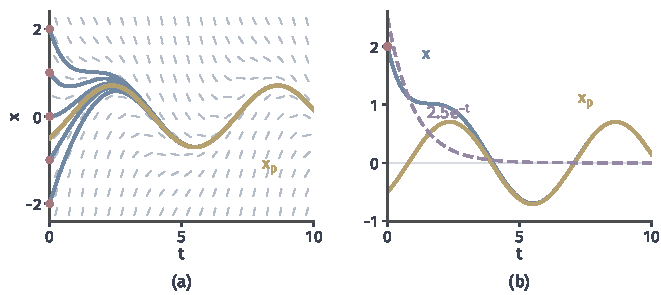
\includegraphics[width=112mm]{figures/06-differential-equations/01-ordinary-differential-equations/matplotlib/lde-first-order-family/figure.pdf}
  \caption{方程$\dot{x}=-x+\sin t$的解族与分解。(a)灰色短线是方向场，蓝线是初值$x_0=-2,-1,0,1,2$（红点）的解，黄线是特解$x_{\mathrm{p}}$。(b)$x_0=2$的解（蓝）等于紫色虚线$2.5\mathrm{e}^{-t}$与黄色特解之和。}
  \label{fig:lde-first-order-family}
\end{BookInlineFigure}

\paragraph{积分因子做了什么}
再看一个系数随时间变化的例子，$\dot{x}=-2tx+2t$，$x(0)=x_0$。这里$\int_0^t a=-t^2$，积分因子是$\mu(t)=\mathrm{e}^{t^2}$。令$y=\mu x$，方程变成
\[
 \dot{y}=2t\mathrm{e}^{t^2}.
\]
右端不再依赖状态，积分得到$y(t)=x_0+\mathrm{e}^{t^2}-1$。除以$\mu$，结果是
\[
 x(t)=1+(x_0-1)\mathrm{e}^{-t^2}.
\]

图~\ref{fig:lde-integrating-factor}对比了$x$和$y$两个坐标。原坐标中的解曲线互相靠拢，斜率同时依赖$t$和$x$。换成$y=\mu x$以后，同一时刻各点斜率相同，解曲线彼此只差一个上下平移，积分因此可以直接进行。

可以把$\mu(t)$想成一把随时间伸缩的尺子。齐次部分造成的伸缩被这把尺子抵消，剩下的只有输入的累积。这个类比只对线性方程成立：非线性方程中伸缩率依赖状态本身，不同解需要不同的尺子。

\begin{BookInlineFigure}
  \centering
  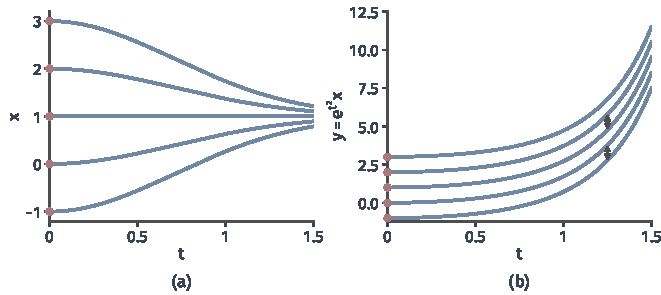
\includegraphics[width=112mm]{figures/06-differential-equations/01-ordinary-differential-equations/matplotlib/lde-integrating-factor/figure.pdf}
  \caption{积分因子的作用，方程$\dot{x}=-2tx+2t$，红点是初值$x_0=-1,0,1,2,3$。(a)原坐标中的解。(b)变量$y=\mathrm{e}^{t^2}x$下，同一批解彼此只差上下平移，黑色双箭头示意相邻两条曲线在同一时刻的间距都是$1$。}
  \label{fig:lde-integrating-factor}
\end{BookInlineFigure}

\paragraph{解的区间由系数决定}
定理~\ref{thm:lde-scalar-solution}要求系数在$I$上连续，$I$之外不作任何保证。考虑$\dot{x}=-x/t+1$，$x(1)=x_0$。系数$a(t)=-1/t$在$t=0$没有定义，初值点$t_0=1$所在的最大连续区间是$I=(0,\infty)$。

由式~\eqref{eq:lde-scalar-propagator}，$\Phi(t,s)=\exp(-\ln t+\ln s)=s/t$。代入式~\eqref{eq:lde-scalar-solution}，
\[
 x(t)=\frac{x_0}{t}+\int_1^t\frac{s}{t}\,\mathrm{d}s=\frac{x_0}{t}+\frac{t^2-1}{2t}.
\]
令$c=x_0-1/2$，解化成
\[
 x(t)=\frac{c}{t}+\frac{t}{2},\qquad t\in(0,\infty).
\]

图~\ref{fig:lde-singular-coefficient}中，$c\neq0$的解在$t\to0^+$时无界，$c=0$的解$x=t/2$却可以一直延伸到$t=0$。这里的奇异位置$t=0$由系数决定，所有解都在同一处遇到它；而$\dot{x}=x^2$的爆炸时刻随初值变化。线性方程的解走不出系数的连续区间，也只有在这个边界上才可能失控。

\begin{BookInlineFigure}
  \centering
  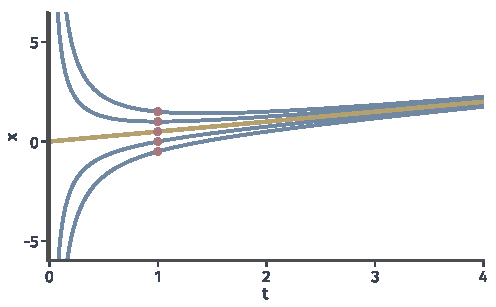
\includegraphics[width=84mm]{figures/06-differential-equations/01-ordinary-differential-equations/matplotlib/lde-singular-coefficient/figure.pdf}
  \caption{系数决定解的区间。方程$\dot{x}=-x/t+1$的解$x=c/t+t/2$，红点是$t=1$处的初值，蓝线取$c=\pm1,\pm0.5$，黄线取$c=0$。左侧深灰粗线$t=0$处系数$-1/t$无定义，所有$c\neq0$的解都在此无界。}
  \label{fig:lde-singular-coefficient}
\end{BookInlineFigure}

\paragraph{可积系数}
第~\ref{chap:ordinary-differential-equations}章说明过，系数或输入只是可测时，解未必处处可微，要用积分形式理解。对线性方程，这种解的含义是：$x$在$I$的每个紧子区间上绝对连续，在$I$上几乎处处满足微分方程，并且$x(t_0)=x_0$。与之等价的写法是
\begin{equation}
 x(t)=x_0+\int_{t_0}^{t}\bigl(a(s)x(s)+g(s)\bigr)\,\mathrm{d}s,\qquad t\in I.
 \label{eq:lde-scalar-integral}
\end{equation}
绝对连续函数的导数几乎处处存在且可积，并能积分回原函数，可参考\BookChapterRef{chap:integration}{卷四第6章“积分”}。

\begin{theorem}[可积系数的一阶线性方程]
\label{thm:lde-scalar-integrable}
设$a,g$在$I$的每个紧子区间上Lebesgue可积，$t_0\in I$。则式~\eqref{eq:lde-scalar-solution}定义的函数是积分方程~\eqref{eq:lde-scalar-integral}在$I$上的唯一局部绝对连续解。
\end{theorem}

\begin{proof}
此时$b(t)=\int_{t_0}^ta$局部绝对连续，$\mu=\mathrm{e}^{-b}$是绝对连续函数与光滑函数的复合，在紧子区间上$b$有界，所以$\mu$与$1/\mu$都局部绝对连续，并且几乎处处有$\dot{\mu}=-a\mu$。

先证唯一。设$x$是局部绝对连续解。局部绝对连续函数的乘积仍局部绝对连续，所以$\mu x$局部绝对连续，几乎处处有
\[
 (\mu x)^{\cdot}=\mu(\dot{x}-ax)=\mu g.
\]
$\mu$在紧子区间上有界，$\mu g$可积。对绝对连续函数用微积分基本定理，得$\mu(t)x(t)-x_0=\int_{t_0}^t\mu g$，这正是式~\eqref{eq:lde-scalar-solution}。

再证存在。令$y(t)=x_0+\int_{t_0}^t\mu g$，它局部绝对连续，几乎处处$\dot{y}=\mu g$。令$x=y/\mu$，它局部绝对连续，并且几乎处处
\[
 \dot{x}=\frac{a}{\mu}y+\frac{1}{\mu}\mu g=ax+g.
\]
再积分回去就得到式~\eqref{eq:lde-scalar-integral}。
\end{proof}

公式没有变化，变化的只是它的解释：求导只在几乎处处成立，真正对每一点都成立的是积分形式。图~\ref{fig:lde-integrable-coefficient}给出两种典型情况。

\begin{example}[两种不光滑的系数]
\label{ex:lde-integrable-coefficients}
第一种是系数跳变。取$x(0)=1$，$g=0$，$a(t)=-1$（$0\leq t<1$），$a(t)=-3$（$t\geq1$）。计算$\int_0^t a$，得到
\[
 x(t)=\begin{cases}\mathrm{e}^{-t},&0\leq t\leq1,\\ \mathrm{e}^{-1}\mathrm{e}^{-3(t-1)},&t\geq1.\end{cases}
\]
左导数$-\mathrm{e}^{-1}$与右导数$-3\mathrm{e}^{-1}$在$t=1$不同，解在这一点不可微，其余各点都满足方程。

第二种是系数在端点无界但可积。取$a(t)=-1/(2\sqrt{t})$，$x(0)=1$。由$\int_0^ta=-\sqrt{t}$得
\[
 x(t)=\mathrm{e}^{-\sqrt{t}}.
\]
它在$t>0$满足方程，导数$-\mathrm{e}^{-\sqrt{t}}/(2\sqrt{t})$在$t\to0^+$时趋于$-\infty$。$x$在$t=0$不可微，式~\eqref{eq:lde-scalar-integral}仍然成立。
\end{example}

\begin{BookInlineFigure}
  \centering
  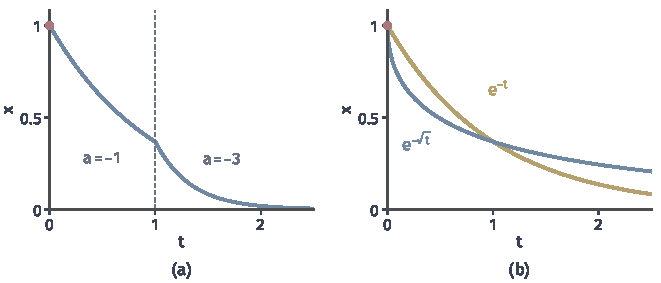
\includegraphics[width=112mm]{figures/06-differential-equations/01-ordinary-differential-equations/matplotlib/lde-integrable-coefficient/figure.pdf}
  \caption{可积系数下的绝对连续解，红点是初值$x(0)=1$。(a)系数在$t=1$从$-1$跳到$-3$，解连续但有折角。(b)系数$-1/(2\sqrt{t})$在$0$处无界但可积，解$\mathrm{e}^{-\sqrt{t}}$（蓝）在$0$处切线竖直；黄线$\mathrm{e}^{-t}$作对照，它在$0$处斜率有限。}
  \label{fig:lde-integrable-coefficient}
\end{BookInlineFigure}


\section{常系数方程}
\label{sec:lde-constant}

一个未知函数不够用时，状态就成了向量。设$\bm{A}\in\mathbb{R}^{n\times n}$是常数矩阵，考虑
\begin{equation}
 \dot{\bm{x}}(t)=\bm{A}\bm{x}(t),\qquad \bm{x}(t_0)=\bm{x}_0.
 \label{eq:lde-constant-system}
\end{equation}
标量情形的解是$\mathrm{e}^{(t-t_0)a}x_0$。向量情形需要回答：矩阵的“指数”是什么，它为什么能解方程，又怎样算出来？高阶标量方程随后会放进同一框架。

\subsection{矩阵指数解}
\label{sec:lde-matrix-exponential}

指数函数的幂级数只用到加法、数乘和乘幂，这些运算对方阵都有定义。于是把级数中的数$a$换成矩阵$\bm{A}$。

\begin{definition}[矩阵指数]
\label{def:lde-matrix-exponential}
对$\bm{A}\in\mathbb{R}^{n\times n}$和$t\in\mathbb{R}$，定义\term{矩阵指数}（matrix exponential）
\begin{equation}
 \mathrm{e}^{t\bm{A}}=\sum_{k=0}^{\infty}\frac{t^k\bm{A}^k}{k!}=\bm{I}+t\bm{A}+\frac{t^2\bm{A}^2}{2}+\cdots.
 \label{eq:lde-matrix-exponential}
\end{equation}
\end{definition}

下面的性质逐条对应标量指数的性质，只有第4条多了一个可交换的条件。

\begin{theorem}[矩阵指数的基本性质]
\label{thm:lde-matexp-properties}
设$\bm{A},\bm{B}\in\mathbb{R}^{n\times n}$，$s,t\in\mathbb{R}$。
\begin{enumerate}
 \item 级数~\eqref{eq:lde-matrix-exponential}绝对收敛，在$t$的有界集上一致收敛，并且
 \begin{equation}
  \lVert\mathrm{e}^{t\bm{A}}\rVert_2\leq\mathrm{e}^{\lvert t\rvert\lVert\bm{A}\rVert_2}.
  \label{eq:lde-matexp-bound}
 \end{equation}
 \item $\mathrm{e}^{0\bm{A}}=\bm{I}$，并且
 \begin{equation}
  \frac{\mathrm{d}}{\mathrm{d}t}\mathrm{e}^{t\bm{A}}=\bm{A}\mathrm{e}^{t\bm{A}}=\mathrm{e}^{t\bm{A}}\bm{A}.
  \label{eq:lde-matexp-derivative}
 \end{equation}
 \item 指数律成立，特别地，$\mathrm{e}^{t\bm{A}}$可逆，逆矩阵是$\mathrm{e}^{-t\bm{A}}$：
 \begin{equation}
  \mathrm{e}^{(t+s)\bm{A}}=\mathrm{e}^{t\bm{A}}\mathrm{e}^{s\bm{A}}.
  \label{eq:lde-matexp-group}
 \end{equation}
 \item 若$\bm{A}\bm{B}=\bm{B}\bm{A}$，则
 \begin{equation}
  \mathrm{e}^{t(\bm{A}+\bm{B})}=\mathrm{e}^{t\bm{A}}\mathrm{e}^{t\bm{B}}.
  \label{eq:lde-matexp-commuting}
 \end{equation}
 \item 若$\bm{V}$可逆，则
 \begin{equation}
  \mathrm{e}^{t\bm{V}\bm{B}\bm{V}^{-1}}=\bm{V}\mathrm{e}^{t\bm{B}}\bm{V}^{-1}.
  \label{eq:lde-matexp-similarity}
 \end{equation}
\end{enumerate}
\end{theorem}

\begin{proof}
(1)谱范数满足$\lVert\bm{A}^k\rVert_2\leq\lVert\bm{A}\rVert_2^k$，所以第$k$项的范数不超过$(\lvert t\rvert\lVert\bm{A}\rVert_2)^k/k!$。当$\lvert t\rvert\leq T$时，它被收敛的数值级数$\sum_k(T\lVert\bm{A}\rVert_2)^k/k!$的通项控制，一致收敛由优级数判别法得到。对这个不等式求和就是所述范数界。

(2)$t=0$时只剩首项$\bm{I}$。逐项求导得到
\[
 \sum_{k\geq1}\frac{t^{k-1}\bm{A}^k}{(k-1)!}=\bm{A}\sum_{j\geq0}\frac{t^{j}\bm{A}^{j}}{j!}.
\]
由(1)，导数级数在有界集上一致收敛，所以逐项求导合法。矩阵$\bm{A}$可以提到左边，也可以提到右边，因为它与自身的乘幂可交换。

(3)固定$s$，定义
\[
 \bm{Y}(t)=\mathrm{e}^{-t\bm{A}}\mathrm{e}^{(t+s)\bm{A}}.
\]
由(2)，
\[
 \dot{\bm{Y}}(t)=-\mathrm{e}^{-t\bm{A}}\bm{A}\mathrm{e}^{(t+s)\bm{A}}+\mathrm{e}^{-t\bm{A}}\bm{A}\mathrm{e}^{(t+s)\bm{A}}=\bm{0}.
\]
所以$\bm{Y}(t)=\bm{Y}(0)=\mathrm{e}^{s\bm{A}}$。取$s=0$得$\mathrm{e}^{-t\bm{A}}\mathrm{e}^{t\bm{A}}=\bm{I}$，方阵的左逆即逆。再用这个逆乘$\bm{Y}(t)=\mathrm{e}^{s\bm{A}}$的两边，就得到加法公式。

(4)$\bm{B}$与$\bm{A}$的每个乘幂可交换，所以$\bm{B}$与$\mathrm{e}^{t\bm{A}}$可交换。定义
\[
 \bm{Y}(t)=\mathrm{e}^{-t(\bm{A}+\bm{B})}\mathrm{e}^{t\bm{A}}\mathrm{e}^{t\bm{B}}.
\]
乘积求导得三项：
\[
 \dot{\bm{Y}}=\mathrm{e}^{-t(\bm{A}+\bm{B})}\bigl(-(\bm{A}+\bm{B})\mathrm{e}^{t\bm{A}}+\bm{A}\mathrm{e}^{t\bm{A}}+\mathrm{e}^{t\bm{A}}\bm{B}\bigr)\mathrm{e}^{t\bm{B}}.
\]
括号内由交换关系等于零，$\bm{Y}(t)=\bm{Y}(0)=\bm{I}$。再用(3)的逆矩阵乘回去。

(5)乘幂满足下式，其中相邻的$\bm{V}^{-1}\bm{V}$都消去了：
\[
 (\bm{V}\bm{B}\bm{V}^{-1})^k=\bm{V}\bm{B}^k\bm{V}^{-1}.
\]
代入级数，提出$\bm{V}$和$\bm{V}^{-1}$。
\end{proof}

\begin{theorem}[常系数齐次系统的解]
\label{thm:lde-constant-solution}
对任意$\bm{x}_0\in\mathbb{R}^n$，初值问题~\eqref{eq:lde-constant-system}在$\mathbb{R}$上有唯一解，它是
\begin{equation}
 \bm{x}(t)=\mathrm{e}^{(t-t_0)\bm{A}}\bm{x}_0.
 \label{eq:lde-constant-solution}
\end{equation}
\end{theorem}

\begin{proof}
由定理~\ref{thm:lde-matexp-properties}的(2)，式~\eqref{eq:lde-constant-solution}满足方程，$t=t_0$时等于$\bm{x}_0$。

反过来设$\bm{x}$是任意一个解，令$\bm{z}(t)=\mathrm{e}^{-(t-t_0)\bm{A}}\bm{x}(t)$。求导得
\[
 \dot{\bm{z}}=\mathrm{e}^{-(t-t_0)\bm{A}}(-\bm{A}\bm{x}+\dot{\bm{x}})=\bm{0}.
\]
所以$\bm{z}(t)=\bm{z}(t_0)=\bm{x}_0$，再乘$\mathrm{e}^{(t-t_0)\bm{A}}$就得到式~\eqref{eq:lde-constant-solution}。
\end{proof}

这个证明与积分因子完全平行：$\mathrm{e}^{-(t-t_0)\bm{A}}$扮演积分因子的角色，它和$\bm{A}$可交换，所以能够抵消方程右端。第~\ref{sec:lde-time-varying}节会看到，时变系数之所以困难，正是因为这种交换关系消失了。

先用级数算一个例子。取
\[
 \bm{J}_0=\begin{bmatrix}0&1\\-1&0\end{bmatrix},
\]
方程是$\dot{x}_1=x_2$、$\dot{x}_2=-x_1$。计算$\bm{J}_0^2=-\bm{I}$，级数的偶次项和奇次项分别凑成余弦和正弦：
\[
 \mathrm{e}^{t\bm{J}_0}=(\cos t)\bm{I}+(\sin t)\bm{J}_0=\begin{bmatrix}\cos t&\sin t\\-\sin t&\cos t\end{bmatrix}.
\]
矩阵的指数在这里是顺时针旋转。图~\ref{fig:lde-matexp-series}(a)画出从$(1,0)^{\top}$出发的轨道和截断到第$K$项的部分和。$K$越大，部分和贴住单位圆的时间越长。

图(b)是固定时刻的截断误差。余项首项的大小约为$t^{K+1}/(K+1)!$，$K$小于$t$时这一项还在增大，超过$t$之后才因阶乘而迅速下降，所以$t$越大需要的项数越多。

\begin{BookInlineFigure}
  \centering
  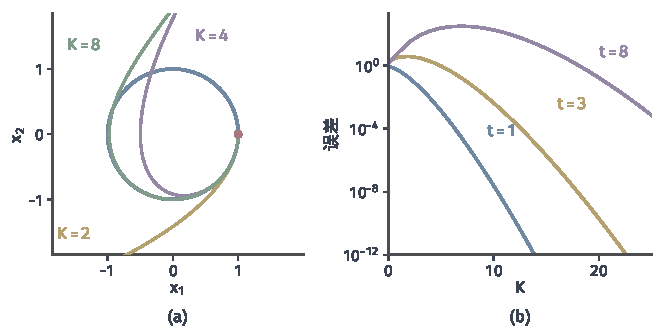
\includegraphics[width=112mm]{figures/06-differential-equations/01-ordinary-differential-equations/matplotlib/lde-matexp-series/figure.pdf}
  \caption{旋转矩阵$\bm{J}_0$的指数级数。(a)蓝色单位圆是精确轨道$\mathrm{e}^{t\bm{J}_0}(1,0)^{\top}$，彩色曲线是$t\in[0,1.5\pi]$上截断到第$K$项的部分和。(b)部分和与$\mathrm{e}^{t\bm{J}_0}$之差的谱范数，纵轴为对数，取$t=1,3,8$。}
  \label{fig:lde-matexp-series}
\end{BookInlineFigure}

\paragraph{对角化：解耦成独立的模式}
级数说明了矩阵指数是什么，计算时却要依靠矩阵的结构。若$\bm{A}$有$n$个线性无关的特征向量，就有$\bm{A}=\bm{V}\bm{\Lambda}\bm{V}^{-1}$，其中$\bm{V}$的列是特征向量$\bm{v}_i$，$\bm{\Lambda}$是特征值组成的对角阵。令$\bm{y}=\bm{V}^{-1}\bm{x}$，方程解耦成$n$个互不相干的标量方程：
\[
 \dot{y}_i=\lambda_iy_i,\qquad i=1,\ldots,n.
\]

记$\bm{w}_i^{\top}$为$\bm{V}^{-1}$的第$i$行。由定理~\ref{thm:lde-matexp-properties}的(5)和对角阵的指数，
\begin{equation}
 \mathrm{e}^{t\bm{A}}=\bm{V}\mathrm{e}^{t\bm{\Lambda}}\bm{V}^{-1}=\sum_{i=1}^{n}\mathrm{e}^{\lambda_it}\bm{v}_i\bm{w}_i^{\top}.
 \label{eq:lde-spectral-exponential}
\end{equation}
读法是：$\bm{w}_i^{\top}\bm{x}_0$量出初值在第$i$个特征方向上的分量，这个分量沿自己的方向按$\mathrm{e}^{\lambda_it}$变化。对角化以及下面用到的三角化（Schur形）的条件与计算，可参考\BookChapterRef{chap:eigen-spectral-decomposition}{卷二第6章“谱分解”}。

\begin{example}[贯穿全章的二维系统]
\label{ex:lde-running-system}
取
\[
 \bm{A}=\begin{bmatrix}0&1\\-2&-3\end{bmatrix}.
\]
特征多项式是$z^2+3z+2=(z+1)(z+2)$，特征值为$-1$和$-2$。解$(\bm{A}-\lambda\bm{I})\bm{v}=\bm{0}$，得到特征向量和它们组成的矩阵：
\[
 \bm{V}=\begin{bmatrix}1&1\\-1&-2\end{bmatrix},\qquad \bm{V}^{-1}=\begin{bmatrix}2&1\\-1&-1\end{bmatrix}.
\]
所以$\bm{w}_1^{\top}=(2,1)$，$\bm{w}_2^{\top}=(-1,-1)$。代入式~\eqref{eq:lde-spectral-exponential}，
\[
 \mathrm{e}^{t\bm{A}}=\mathrm{e}^{-t}\begin{bmatrix}2&1\\-2&-1\end{bmatrix}+\mathrm{e}^{-2t}\begin{bmatrix}-1&-1\\2&2\end{bmatrix}.
\]
取$t=0$，两个矩阵相加恰为$\bm{I}$，这是一次检验。取$\bm{x}_0=(1,0)^{\top}$，第一列给出
\[
 x_1(t)=2\mathrm{e}^{-t}-\mathrm{e}^{-2t},\qquad x_2(t)=-2\mathrm{e}^{-t}+2\mathrm{e}^{-2t}.
\]
再检验方程：$\dot{x}_1=-2\mathrm{e}^{-t}+2\mathrm{e}^{-2t}=x_2$，$\dot{x}_2=2\mathrm{e}^{-t}-4\mathrm{e}^{-2t}$，而
\[
 -2x_1-3x_2=2\mathrm{e}^{-t}-4\mathrm{e}^{-2t}.
\]
\end{example}

图~\ref{fig:lde-diagonal-modes}把同一批初值放在两个坐标系中。(a)的轨线弯曲，看不出规律；(b)用特征坐标后，两个坐标各自按$\mathrm{e}^{-t}$和$\mathrm{e}^{-2t}$收缩。$y_2$衰减得更快，所以轨线在到达原点前几乎都贴向$y_1$轴，在原坐标中表现为贴向$\bm{v}_1$方向。

\begin{BookInlineFigure}
  \centering
  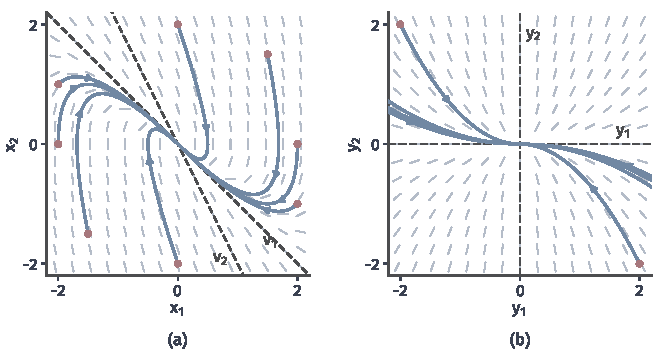
\includegraphics[width=112mm]{figures/06-differential-equations/01-ordinary-differential-equations/matplotlib/lde-diagonal-modes/figure.pdf}
  \caption{对角化解耦，系统取例~\ref{ex:lde-running-system}的$\bm{A}$。(a)原坐标的相平面，灰色短线是方向，蓝线是解，红点是初值，深灰虚线是特征方向$\bm{v}_1,\bm{v}_2$。(b)特征坐标$\bm{y}=\bm{V}^{-1}\bm{x}$中同一批解（超出显示范围的初值点未标出），特征方向成为坐标轴。}
  \label{fig:lde-diagonal-modes}
\end{BookInlineFigure}

\paragraph{复特征值：旋转与伸缩}
实矩阵可能有共轭复特征值$\alpha\pm\mathrm{i}\beta$（$\beta\neq0$）。式~\eqref{eq:lde-spectral-exponential}在复数域上仍然成立，但实系统的解是实的，更好的写法是看典型的二维块
\[
 \bm{A}=\begin{bmatrix}\alpha&\beta\\-\beta&\alpha\end{bmatrix}=\alpha\bm{I}+\beta\bm{J}_0.
\]
$\alpha\bm{I}$与任何矩阵可交换，由定理~\ref{thm:lde-matexp-properties}的(4)，
\begin{equation}
 \mathrm{e}^{t\bm{A}}=\mathrm{e}^{\alpha t}\begin{bmatrix}\cos\beta t&\sin\beta t\\-\sin\beta t&\cos\beta t\end{bmatrix}.
 \label{eq:lde-complex-block}
\end{equation}
实部$\alpha$负责伸缩，虚部$\beta$负责旋转的快慢。图~\ref{fig:lde-spiral}取$\alpha=-1$、$\beta=2$：相平面上是向内的螺线，分量则是被$\pm\mathrm{e}^{-t}$夹住的振荡。一般实矩阵的共轭特征值对，可以用实的相似变换化成这种二维块。

\begin{BookInlineFigure}
  \centering
  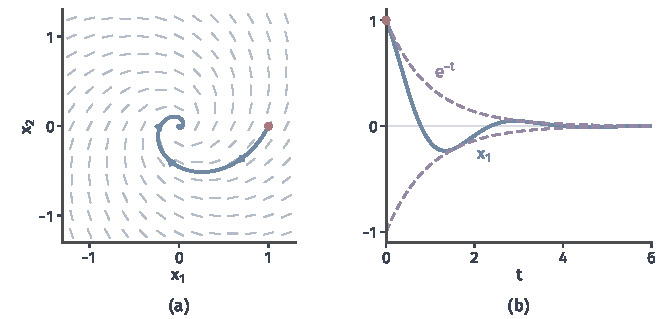
\includegraphics[width=112mm]{figures/06-differential-equations/01-ordinary-differential-equations/matplotlib/lde-spiral/figure.pdf}
  \caption{复特征值对应旋转与伸缩，$\bm{A}=\left[\begin{smallmatrix}-1&2\\-2&-1\end{smallmatrix}\right]$，特征值$-1\pm2\mathrm{i}$，初值$(1,0)^{\top}$（红点）。(a)相平面的螺线。(b)分量$x_1=\mathrm{e}^{-t}\cos2t$（蓝）与紫色虚线包络$\pm\mathrm{e}^{-t}$。}
  \label{fig:lde-spiral}
\end{BookInlineFigure}

\paragraph{三角形式：逐行回代}
不能对角化时，总可以退到三角形式。任意复方阵都酉相似于上三角阵$\bm{T}$，对角元是全部特征值；定理~\ref{thm:lde-matexp-properties}对复矩阵同样成立，证明不变。上三角系统的最后一行不含其他分量，可以先解出；倒数第二行以它为输入，又是一个一阶线性方程。于是第~\ref{sec:lde-first-order}节的公式可以逐行使用。

看一个具体的矩阵：
\[
 \bm{A}=\begin{bmatrix}-1&1\\0&-2\end{bmatrix}.
\]
第二行给出$x_2(t)=\mathrm{e}^{-2t}x_2(0)$。第一行是$\dot{x}_1=-x_1+x_2$，由式~\eqref{eq:lde-scalar-solution}，
\[
 x_1(t)=\mathrm{e}^{-t}x_1(0)+\Bigl(\int_0^t\mathrm{e}^{-(t-s)}\mathrm{e}^{-2s}\,\mathrm{d}s\Bigr)x_2(0).
\]
括号内的积分提出$\mathrm{e}^{-t}$后等于
\[
 \mathrm{e}^{-t}\int_0^t\mathrm{e}^{-s}\,\mathrm{d}s=\mathrm{e}^{-t}-\mathrm{e}^{-2t},
\]
所以
\[
 x_1(t)=\mathrm{e}^{-t}x_1(0)+(\mathrm{e}^{-t}-\mathrm{e}^{-2t})x_2(0).
\]

现在把第二个对角元也改成$-1$。积分变成$\int_0^t\mathrm{e}^{-(t-s)}\mathrm{e}^{-s}\,\mathrm{d}s$，被积函数恒等于$\mathrm{e}^{-t}$，与$s$无关，积分结果是$t\mathrm{e}^{-t}$。多项式因子就这样出现了：上一行的输出含有与下一行自身相同的模式，贡献按时间不断累积，而不是像前一例那样互相抵消。

\paragraph{Jordan块：不能只看特征值}
比较两个$2\times2$矩阵$-\bm{I}$和
\[
 \bm{J}=\begin{bmatrix}-1&1\\0&-1\end{bmatrix}.
\]
它们的特征多项式都是$(z+1)^2$，特征值完全相同，指数却不同。一般地，形如$\lambda\bm{I}+\bm{N}$的$s$阶矩阵称为Jordan块，其中$\bm{N}$的超对角元为$1$、其余元素为$0$，满足$\bm{N}^s=\bm{0}$。$\lambda\bm{I}$与$\bm{N}$可交换，由定理~\ref{thm:lde-matexp-properties}的(4)，级数在第$s$项截断：
\begin{equation}
 \mathrm{e}^{t(\lambda\bm{I}+\bm{N})}=\mathrm{e}^{\lambda t}\sum_{j=0}^{s-1}\frac{t^j\bm{N}^j}{j!}.
 \label{eq:lde-jordan-exponential}
\end{equation}

对上面的$\bm{J}$，$s=2$，结果是
\[
 \mathrm{e}^{t\bm{J}}=\mathrm{e}^{-t}\begin{bmatrix}1&t\\0&1\end{bmatrix},
\]
而$\mathrm{e}^{-t\bm{I}}=\mathrm{e}^{-t}\bm{I}$没有$t$项。二者的差别在于特征向量的个数。$-\bm{I}$的特征向量张成整个平面，$\bm{J}$只有$\bm{e}_1$一个方向。卷二讨论矩阵幂时已经遇到同样的现象，$\bm{J}^k$中出现了$k$的多项式因子，可参考\BookChapterRef{chap:linear-recurrence-stability}{卷二第10章“线性递推的收敛与稳定性”}。

缺少的方向由\term{广义特征向量}（generalized eigenvector）补上：满足$(\bm{A}-\lambda\bm{I})^2\bm{v}=\bm{0}$而$\bm{u}=(\bm{A}-\lambda\bm{I})\bm{v}\neq\bm{0}$的向量$\bm{v}$。此时$\bm{u}$是特征向量，并且从$\bm{v}$出发的解是
\begin{equation}
 \bm{x}(t)=\mathrm{e}^{\lambda t}\bigl(\bm{v}+t\bm{u}\bigr).
 \label{eq:lde-generalized-solution}
\end{equation}
对$\bm{J}$取$\bm{v}=\bm{e}_2$，则$\bm{u}=\bm{e}_1$，式~\eqref{eq:lde-generalized-solution}与$\mathrm{e}^{t\bm{J}}$的第二列一致。

图~\ref{fig:lde-jordan-vs-diagonal}把差别画了出来。(a)中每条轨线都是直线，(b)中轨线都沿唯一的特征方向进入原点，看起来像被拧过。图~\ref{fig:lde-jordan-chain}给出多项式因子的另一种读法：Jordan块是一串相同的一阶系统首尾相接，每经过一级，就多累积一次，多一个$t$的幂。

\begin{BookInlineFigure}
  \centering
  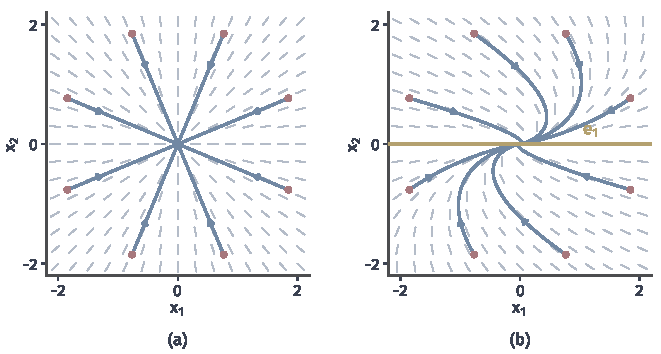
\includegraphics[width=112mm]{figures/06-differential-equations/01-ordinary-differential-equations/matplotlib/lde-jordan-vs-diagonal/figure.pdf}
  \caption{特征值相同而相图不同，红点是半径为$2$的圆上的初值。(a)$\bm{A}=-\bm{I}$，每个方向都是特征方向，轨线是直线。(b)$\bm{A}=\bm{J}$，只有黄色的$\bm{e}_1$轴是特征方向，其余轨线都沿它的方向进入原点。}
  \label{fig:lde-jordan-vs-diagonal}
\end{BookInlineFigure}

\begin{BookInlineFigure}
  \centering
  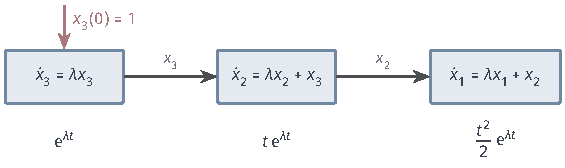
\includegraphics[width=96mm]{figures/06-differential-equations/01-ordinary-differential-equations/tikz/lde-jordan-chain/figure.pdf}
  \caption{三阶Jordan块看作一阶系统的串联。方框中是三个分量的方程，红色箭头表示只给$x_3$非零初值，方框下方是相应分量的响应。每一级的输入都含有该级自身的模式$\mathrm{e}^{\lambda t}$，于是响应多一次累积，得到$t$的更高次幂。}
  \label{fig:lde-jordan-chain}
\end{BookInlineFigure}

只看特征值还会错过有限时间内的放大。取
\[
 \bm{A}=\begin{bmatrix}-1&10\\0&-1\end{bmatrix},\qquad \bm{x}_0=\begin{bmatrix}0\\1\end{bmatrix}.
\]
把$\bm{N}$换成$10\bm{N}$，式~\eqref{eq:lde-jordan-exponential}给出
\[
 x_1(t)=10t\mathrm{e}^{-t},\qquad x_2(t)=\mathrm{e}^{-t}.
\]
两个特征值都是$-1$，看上去每个模式都在衰减，$x_1$却从$0$升到$t=1$处的$10/\mathrm{e}\approx3.68$，然后才下降，见图~\ref{fig:lde-jordan-transient}。放大来自对角线上方的耦合，特征值感受不到它。

\begin{BookInlineFigure}
  \centering
  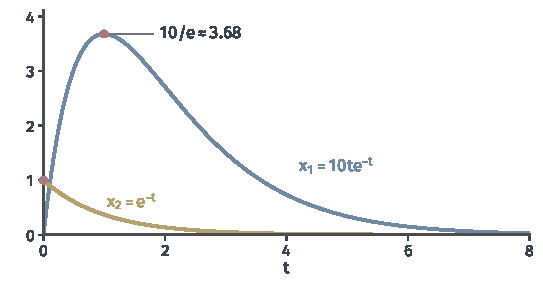
\includegraphics[width=92mm]{figures/06-differential-equations/01-ordinary-differential-equations/matplotlib/lde-jordan-transient/figure.pdf}
  \caption{重特征值带来的有限时间放大。$\bm{A}=\left[\begin{smallmatrix}-1&10\\0&-1\end{smallmatrix}\right]$，$\bm{x}_0=(0,1)^{\top}$。蓝线是$x_1$，在$t=1$达到峰值（右侧红点）；黄线是$x_2$，从左侧红点单调下降。}
  \label{fig:lde-jordan-transient}
\end{BookInlineFigure}

\paragraph{解的一般形状}
三角形式的回代可以写成一个对所有矩阵都成立的结论。

\begin{theorem}[矩阵指数的元素]
\label{thm:lde-exponential-shape}
设$\bm{A}\in\mathbb{R}^{n\times n}$的互异特征值为$\lambda_1,\ldots,\lambda_r$，代数重数为$m_1,\ldots,m_r$。则$\mathrm{e}^{t\bm{A}}$的每个元素都是下列函数的线性组合：
\begin{equation}
 t^j\mathrm{e}^{\lambda_it},\qquad 0\leq j<m_i,\quad i=1,\ldots,r.
 \label{eq:lde-exponential-shape}
\end{equation}
组合系数一般是复数。
\end{theorem}

\begin{proof}
由定理~\ref{thm:lde-matexp-properties}的(5)，只需证明上三角阵$\bm{T}$的情形。设$\bm{T}$的对角元为$\tau_1,\ldots,\tau_n$，解$\dot{\bm{x}}=\bm{T}\bm{x}$。从$i=n$往回归纳，证明$x_i$是若干$t^j\mathrm{e}^{\lambda t}$的组合，其中$\lambda\in\{\tau_i,\ldots,\tau_n\}$，$j$小于$\lambda$在$\tau_i,\ldots,\tau_n$中出现的次数。

$i=n$时$x_n=\mathrm{e}^{\tau_nt}x_n(0)$。设结论对$i+1,\ldots,n$成立。第$i$行是以$\sum_{k>i}T_{i,k}x_k$为输入的一阶线性方程，所以只要看一项输入$s^j\mathrm{e}^{\lambda s}$产生什么：
\[
 \int_0^t\mathrm{e}^{\tau_i(t-s)}s^j\mathrm{e}^{\lambda s}\,\mathrm{d}s=\mathrm{e}^{\tau_it}\int_0^ts^j\mathrm{e}^{(\lambda-\tau_i)s}\,\mathrm{d}s.
\]
若$\lambda\neq\tau_i$，分部积分$j$次得到次数至多为$j$的多项式乘$\mathrm{e}^{\lambda t}$，再加常数乘$\mathrm{e}^{\tau_it}$，幂次不升。若$\lambda=\tau_i$，积分等于$t^{j+1}/(j+1)$，幂次升一，而$\tau_i$在列表中恰好多出现一次。两种情形都保持归纳假设。
\end{proof}

定理说明指数、振荡和多项式因子是常系数线性系统仅有的三种成分：实部给出指数，虚部给出振荡，重根可能给出多项式。这里的“可能”不能省略，$-\bm{I}$就没有多项式因子。利用Jordan标准形可以把幂次上限收紧为“$j$小于$\lambda_i$的最大Jordan块阶数”，Jordan标准形的存在性证明较长，读者可查阅线性代数教材。

特征值的实部决定解在$t\to\infty$时的走向，但判断长期稳定还要考虑实部为零的特征值和Jordan块的大小，也要处理非线性系统，相关判据可参考\BookChapterRef{chap:dynamical-systems-long-term}{卷九第1章“动力系统与轨迹的长期行为”}。本章只关心解在有限时间上的形状。

\subsection{高阶标量方程}
\label{sec:lde-high-order}

质点在弹簧上的振动由二阶方程描述，电路和梁的问题还会出现更高阶的方程。记$\mathrm{D}=\mathrm{d}/\mathrm{d}t$，常系数$n$阶线性方程写作
\begin{equation}
 \mathrm{D}^nx+a_{n-1}\mathrm{D}^{n-1}x+\cdots+a_1\mathrm{D}x+a_0x=g(t),
 \label{eq:lde-high-order}
\end{equation}
其中系数$a_0,\ldots,a_{n-1}$是实常数。初值要给齐$x,\mathrm{D}x,\ldots,\mathrm{D}^{n-1}x$在$t_0$的值，共$n$个数。多项式$p(z)=z^n+a_{n-1}z^{n-1}+\cdots+a_0$称为方程的特征多项式，于是方程可以简写成$p(\mathrm{D})x=g$。

\paragraph{状态降阶}
第~\ref{chap:ordinary-differential-equations}章用位移和速度描述摆的状态，高阶方程也一样。令$x_k=\mathrm{D}^{k-1}x$（$k=1,\ldots,n$），前$n-1$个分量的方程就是定义$\dot{x}_k=x_{k+1}$，最后一个分量由方程~\eqref{eq:lde-high-order}解出。写成矩阵形式：
\begin{equation}
 \dot{\bm{x}}=\bm{C}\bm{x}+g(t)\bm{e}_n,\qquad
 \bm{C}=\begin{bmatrix}0&1&&\\&\ddots&\ddots&\\&&0&1\\-a_0&-a_1&\cdots&-a_{n-1}\end{bmatrix}.
 \label{eq:lde-companion}
\end{equation}
$\bm{C}$称为\term{友矩阵}（companion matrix）。例~\ref{ex:lde-running-system}的矩阵正是$p(z)=z^2+3z+2$的友矩阵。

图~\ref{fig:lde-companion-chain}把$n=3$的情形画成积分器串联。每个积分器保存一个状态分量，也就是系统需要“记住”的一个量，这也解释了为什么要给$n$个初值。

\begin{BookInlineFigure}
  \centering
  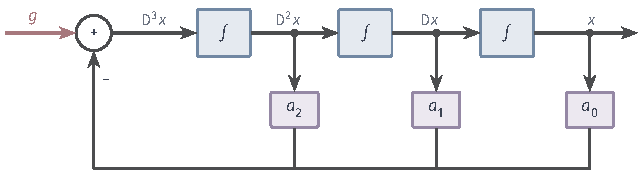
\includegraphics[width=108mm]{figures/06-differential-equations/01-ordinary-differential-equations/tikz/lde-companion-chain/figure.pdf}
  \caption{三阶方程$\mathrm{D}^3x+a_2\mathrm{D}^2x+a_1\mathrm{D}x+a_0x=g$的状态结构。蓝框是积分器，输出依次为状态分量$\mathrm{D}^2x,\mathrm{D}x,x$；紫框是系数，反馈后与红色输入$g$在求和点相减，得到最高阶导数。}
  \label{fig:lde-companion-chain}
\end{BookInlineFigure}

\begin{lemma}[友矩阵的谱]
\label{lem:lde-companion}
$\bm{C}$的特征多项式是$p$。对$\bm{C}$的每个特征值$\lambda$，特征子空间都是一维的，由下面的向量张成：
\begin{equation}
 \bm{v}(\lambda)=(1,\lambda,\lambda^2,\ldots,\lambda^{n-1})^{\top}.
 \label{eq:lde-companion-eigenvector}
\end{equation}
\end{lemma}

\begin{proof}
把$z\bm{I}-\bm{C}$的第$k$列乘$z^{k-1}$加到第$1$列（$k=2,\ldots,n$），行列式不变。逐行计算，新的第$1$列是$(0,\ldots,0,p(z))^{\top}$。

沿第$1$列展开，代数余子式对应的$n-1$阶子矩阵是下三角阵，对角元全为$-1$，行列式为$(-1)^{n-1}$。它再乘符号$(-1)^{n+1}$，结果是
\[
 \det(z\bm{I}-\bm{C})=(-1)^{n+1}(-1)^{n-1}p(z)=p(z).
\]

设$\bm{C}\bm{v}=\lambda\bm{v}$。前$n-1$行给出$v_{k+1}=\lambda v_k$，所以$\bm{v}$由$v_1$决定，并且$\bm{v}=v_1\bm{v}(\lambda)$。这就是特征子空间的一维性。
\end{proof}

引理的第二部分有直接的后果：若$\lambda$是$p$的$m$重根，$\bm{C}$在$\lambda$上只有一个Jordan块，阶数就是$m$。所以高阶标量方程不可能出现$-\bm{I}$那样“重特征值却没有多项式因子”的情况，重根一定带来$t,\ldots,t^{m-1}$。

\paragraph{基本解的列表}
上面的结论也可以直接从算子分解得到。常系数算子彼此可交换，$p(\mathrm{D})$可按根分解。关键的计算只有一步：
\[
 (\mathrm{D}-\lambda)\bigl(t^j\mathrm{e}^{\lambda t}\bigr)=jt^{j-1}\mathrm{e}^{\lambda t}.
\]
每作用一次$\mathrm{D}-\lambda$，$t$的幂次降一，所以$(\mathrm{D}-\lambda)^m$把$t^j\mathrm{e}^{\lambda t}$（$j<m$）变成零。

\begin{theorem}[高阶齐次方程的基本解]
\label{thm:lde-high-order-basis}
设$p(z)=\prod_{i=1}^{r}(z-\lambda_i)^{m_i}$，$\lambda_i$互异，$\sum_im_i=n$。则方程$p(\mathrm{D})x=0$的复值解构成$n$维线性空间，下列$n$个函数是它的一组基：
\begin{equation}
 t^j\mathrm{e}^{\lambda_it},\qquad 0\leq j<m_i,\quad i=1,\ldots,r.
 \label{eq:lde-high-order-basis}
\end{equation}
系数为实数时，一对共轭根$\alpha\pm\mathrm{i}\beta$对应的函数可以换成实函数$t^j\mathrm{e}^{\alpha t}\cos\beta t$和$t^j\mathrm{e}^{\alpha t}\sin\beta t$。
\end{theorem}

\begin{proof}
由上面的计算，这$n$个函数都是解。解空间的维数是$n$：由定理~\ref{thm:lde-constant-solution}，把解对应到初始状态$(x(0),\ldots,\mathrm{D}^{n-1}x(0))$是线性双射。

只需证明线性无关。假设存在非平凡关系$\sum_{i=1}^{r}q_i(t)\mathrm{e}^{\lambda_it}=0$，其中多项式$q_i$都不为零，$\lambda_i$互异，并取其中$r$最小的一个。$r=1$时$q_1\equiv0$，矛盾。

设$r\geq2$。乘$\mathrm{e}^{-\lambda_rt}$，再求导$\deg q_r+1$次，把$q_r$消去。其余每一项形如$q\mathrm{e}^{\mu t}$，$\mu=\lambda_i-\lambda_r\neq0$，而
\[
 \mathrm{D}(q\mathrm{e}^{\mu t})=(\dot{q}+\mu q)\mathrm{e}^{\mu t}.
\]
多项式的次数不变，首项系数乘$\mu$。所以得到一个只有$r-1$个指数的非平凡关系，与$r$的最小性矛盾。

系数为实数时，共轭根成对出现且重数相同。$t^j\mathrm{e}^{\alpha t}\cos\beta t$和$t^j\mathrm{e}^{\alpha t}\sin\beta t$分别是$t^j\mathrm{e}^{(\alpha\pm\mathrm{i}\beta)t}$的半和与半差（后者再除以$\mathrm{i}$），两组函数张成同一个空间。
\end{proof}

\paragraph{二阶振动方程}
质点受弹簧恢复力和阻尼时，满足$\ddot{x}+b\dot{x}+cx=0$，其中$b,c$是正常数。特征方程$z^2+bz+c=0$的判别式把运动分成三类。下面三个例子都取$x(0)=1$、$\dot{x}(0)=0$，只改变根的形状。

实根$p(z)=z^2+3z+2$，根为$-1,-2$。设$x=C_1\mathrm{e}^{-t}+C_2\mathrm{e}^{-2t}$，初值给出$C_1+C_2=1$和$-C_1-2C_2=0$，于是
\[
 x(t)=2\mathrm{e}^{-t}-\mathrm{e}^{-2t}.
\]

重根$p(z)=z^2+2z+1$，根为$-1$（二重）。设$x=(C_1+C_2t)\mathrm{e}^{-t}$，初值给出$C_1=1$和$-C_1+C_2=0$，于是
\[
 x(t)=(1+t)\mathrm{e}^{-t}.
\]

复根$p(z)=z^2+2z+5$，根为$-1\pm2\mathrm{i}$。设$x=\mathrm{e}^{-t}(C_1\cos2t+C_2\sin2t)$，初值给出$C_1=1$和$-C_1+2C_2=0$，于是
\[
 x(t)=\mathrm{e}^{-t}\Bigl(\cos2t+\frac12\sin2t\Bigr).
\]

图~\ref{fig:lde-damped-cases}比较这三条曲线。实根时质点单调回到平衡位置，复根时越过平衡位置来回摆动。重根恰好是两种情形的分界，它没有越过平衡位置，多项式因子$1+t$让它在开始阶段下降得比实根情形慢。三种情形及其物理名称见表~\ref{tab:lde-second-order}。

\begin{BookInlineFigure}
  \centering
  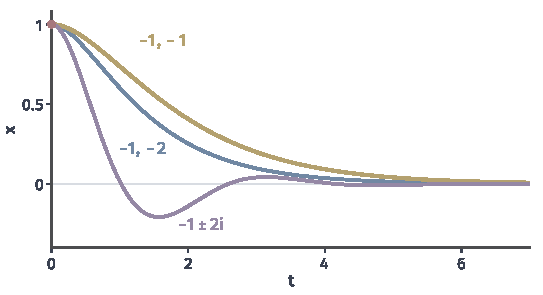
\includegraphics[width=92mm]{figures/06-differential-equations/01-ordinary-differential-equations/matplotlib/lde-damped-cases/figure.pdf}
  \caption{同一初值$x(0)=1$、$\dot{x}(0)=0$（红点）下的三类二阶方程，线旁标注特征根。蓝线：实根$-1,-2$。黄线：重根$-1,-1$。紫线：复根$-1\pm2\mathrm{i}$。}
  \label{fig:lde-damped-cases}
\end{BookInlineFigure}

\begin{BookInlineTable}
  \centering
  \caption{二阶常系数齐次方程的三类根。}
  \label{tab:lde-second-order}
  \begin{tabular}{lll}
    \toprule
    根的形状 & 基本解 & 运动形式\\
    \midrule
    相异实根$\lambda_1,\lambda_2$ & $\mathrm{e}^{\lambda_1t},\ \mathrm{e}^{\lambda_2t}$ & 过阻尼：不振荡\\
    二重根$\lambda$ & $\mathrm{e}^{\lambda t},\ t\mathrm{e}^{\lambda t}$ & 临界阻尼：不振荡的边界\\
    共轭复根$\alpha\pm\mathrm{i}\beta$ & $\mathrm{e}^{\alpha t}\cos\beta t,\ \mathrm{e}^{\alpha t}\sin\beta t$ & 欠阻尼：衰减振荡\\
    \bottomrule
  \end{tabular}
\end{BookInlineTable}

\paragraph{重根是两个根相撞}
重根的$t\mathrm{e}^{\lambda t}$看上去来得突然，用连续变化的系数看却很自然。考虑$\ddot{x}+2c\dot{x}+x=0$，根为$-c\pm\sqrt{c^2-1}$。图~\ref{fig:lde-root-locus}(a)显示，$c$从$0$增大到$1$时，一对共轭根沿单位圆向左靠拢，在$c=1$相撞于$-1$，然后沿实轴分开。

相撞时两个基本解变成同一个函数，线性无关性似乎丢失了。补救办法是取差商。令两根为$-1$和$-1-\varepsilon$，它们的基本解之差除以$\varepsilon$仍是解，而
\[
 \lim_{\varepsilon\to0}\frac{\mathrm{e}^{-t}-\mathrm{e}^{-(1+\varepsilon)t}}{\varepsilon}=t\mathrm{e}^{-t}.
\]
这个极限就是$\mathrm{e}^{\lambda t}$对$\lambda$的导数。图(b)中$\varepsilon$减小时差商曲线逐步靠近$t\mathrm{e}^{-t}$。两个靠得很近的根已经几乎产生了线性增长的因子，重根只是这个过程的极限。

\begin{BookInlineFigure}
  \centering
  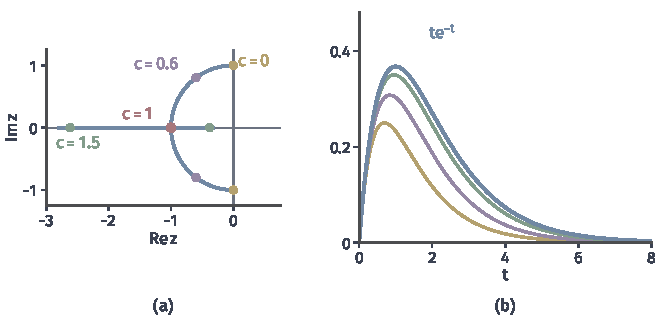
\includegraphics[width=112mm]{figures/06-differential-equations/01-ordinary-differential-equations/matplotlib/lde-root-locus/figure.pdf}
  \caption{根的相撞与多项式因子。(a)$z^2+2cz+1$的根随$c$的移动：$c=0$时在虚轴，$c=0.6$时在单位圆上，$c=1$时相撞于红点，$c=1.5$时分开在实轴上。(b)根为$-1,-1-\varepsilon$时的差商$(\mathrm{e}^{-t}-\mathrm{e}^{-(1+\varepsilon)t})/\varepsilon$，黄、紫、绿线依次取$\varepsilon=1,0.4,0.1$，蓝线是极限$t\mathrm{e}^{-t}$。}
  \label{fig:lde-root-locus}
\end{BookInlineFigure}


\section{时变系统}
\label{sec:lde-time-varying}

系数矩阵随时间变化时，方程变成
\begin{equation}
 \dot{\bm{x}}(t)=\bm{A}(t)\bm{x}(t),\qquad \bm{x}(s)=\bm{\xi},
 \label{eq:lde-time-varying}
\end{equation}
其中$\bm{A}:I\to\mathbb{R}^{n\times n}$在区间$I$上连续，$s\in I$。一个自然的想法是照搬标量公式，用$\exp\int_s^t\bm{A}$作传播。这个想法一般是错的，错在哪里要等传播矩阵本身建立好才能说清。所以先回答：不写闭式，能否定义出从时刻$s$到时刻$t$的线性传播？

\paragraph{用迭代造出传播矩阵}
把方程~\eqref{eq:lde-time-varying}对时间积分，得到
\[
 \bm{x}(t)=\bm{\xi}+\int_s^t\bm{A}(r)\bm{x}(r)\,\mathrm{d}r.
\]
解出现在右端，于是把右端的$\bm{x}$反复用整个等式代入。第一次代入后多出一项，第二次代入后再多一项，一直做下去，得到矩阵的级数
\begin{equation}
 \begin{aligned}
 \bm{\Phi}(t,s)={}&\bm{I}+\int_s^t\bm{A}(r_1)\,\mathrm{d}r_1\\
 &+\int_s^t\!\!\int_s^{r_1}\bm{A}(r_1)\bm{A}(r_2)\,\mathrm{d}r_2\,\mathrm{d}r_1+\cdots,
 \end{aligned}
 \label{eq:lde-peano-baker}
\end{equation}
称为\term{Peano--Baker级数}（Peano--Baker series）。第$k$项是$k$重积分，被积函数中时间较晚的因子写在左边。

这个级数是矩阵指数的时间排序版本。$\bm{A}$是常数时，第$k$项被积函数恒为$\bm{A}^k$，积分区域$s\leq r_k\leq\cdots\leq r_1\leq t$的体积是$(t-s)^k/k!$，第$k$项就是$(t-s)^k\bm{A}^k/k!$，级数回到式~\eqref{eq:lde-matrix-exponential}。阶乘的来历也清楚了：它是$k$个时刻按先后排列的区域在立方体中所占的比例。

\begin{definition}[状态转移矩阵]
\label{def:lde-transition}
设$\bm{A}$在$I$上连续，$s\in I$。把矩阵初值问题
\begin{equation}
 \partial_t\bm{\Phi}(t,s)=\bm{A}(t)\bm{\Phi}(t,s),\qquad \bm{\Phi}(s,s)=\bm{I}
 \label{eq:lde-transition}
\end{equation}
的解称为\term{状态转移矩阵}（state transition matrix）。第一个自变量$t$是终止时刻，第二个自变量$s$是初始时刻。
\end{definition}

\begin{theorem}[线性系统的整体存在唯一]
\label{thm:lde-transition-existence}
设$\bm{A}$在$I$上连续。对每个$s\in I$，问题~\eqref{eq:lde-transition}在整个$I$上有唯一解，由级数~\eqref{eq:lde-peano-baker}给出。对每个$\bm{\xi}\in\mathbb{R}^n$，方程~\eqref{eq:lde-time-varying}在$I$上的唯一解是
\begin{equation}
 \bm{x}(t)=\bm{\Phi}(t,s)\bm{\xi}.
 \label{eq:lde-transition-solution}
\end{equation}
\end{theorem}

\begin{proof}
取含$s$的紧子区间$J\subset I$，定义累积系数大小
\[
 \alpha(t)=\Bigl\lvert\int_s^t\lVert\bm{A}(r)\rVert_2\,\mathrm{d}r\Bigr\rvert.
\]
记级数第$k$项为$\bm{T}_k(t)$，它满足$\bm{T}_0=\bm{I}$和递推关系
\[
 \bm{T}_{k+1}(t)=\int_s^t\bm{A}(r)\bm{T}_k(r)\,\mathrm{d}r.
\]
归纳可得$\lVert\bm{T}_k(t)\rVert_2\leq\alpha(t)^k/k!$，归纳一步是
\[
 \lVert\bm{T}_{k+1}(t)\rVert_2\leq\Bigl\lvert\int_s^t\lVert\bm{A}(r)\rVert_2\frac{\alpha(r)^k}{k!}\,\mathrm{d}r\Bigr\rvert=\frac{\alpha(t)^{k+1}}{(k+1)!}.
\]

$\alpha$在$J$上有界，由优级数判别法，级数在$J$上一致收敛到连续的矩阵函数$\bm{\Phi}(\cdot,s)$。把递推式对$k$求和，并在一致收敛下交换求和与积分，得到
\[
 \bm{\Phi}(t,s)=\bm{I}+\int_s^t\bm{A}(r)\bm{\Phi}(r,s)\,\mathrm{d}r.
\]
被积函数连续，所以$\bm{\Phi}$对$t$连续可微，满足式~\eqref{eq:lde-transition}。$J$可以任取，所以解在整个$I$上存在。

再证唯一。设向量函数$\bm{y}$满足$\dot{\bm{y}}=\bm{A}\bm{y}$、$\bm{y}(s)=\bm{0}$，令$B=\max_J\lVert\bm{y}\rVert_2$。积分形式给出$\lVert\bm{y}(t)\rVert_2\leq B\alpha(t)$，代回积分形式再估计，反复进行，得到对每个$k$都有
\[
 \lVert\bm{y}(t)\rVert_2\leq\frac{B\alpha(t)^k}{k!}.
\]
令$k\to\infty$得$\bm{y}\equiv\bm{0}$。把它用于两个解之差，矩阵方程按列处理，就得到两个问题解的唯一性。式~\eqref{eq:lde-transition-solution}满足方程~\eqref{eq:lde-time-varying}可以直接代入验证。
\end{proof}

第~\ref{chap:ode-existence-continuation}章会把同样的迭代用于非线性方程，那里一般只能得到局部结论。线性方程的估计不受状态大小的影响，所以结论对整个$I$成立。若$\bm{A}$只是分段连续，就在每一段上求解，并在接缝处把状态接起来，$\bm{\Phi}$仍然连续，只是对$t$的导数在接缝处有跳变。

\paragraph{基本解矩阵}
实际求解时，往往是先设法找到$n$个线性无关的解，再组装成传播矩阵。

\begin{definition}[基本解矩阵]
\label{def:lde-fundamental-matrix}
若矩阵函数$\bm{X}:I\to\mathbb{R}^{n\times n}$连续可微，满足下式，并且在某一时刻可逆，就称它为\term{基本解矩阵}（fundamental matrix）：
\begin{equation}
 \dot{\bm{X}}(t)=\bm{A}(t)\bm{X}(t).
 \label{eq:lde-fundamental-matrix}
\end{equation}
\end{definition}

它的$n$列是$n$个解。若$\bm{X}$在某时刻$t_*$可逆，则它在每个时刻都可逆。否则存在时刻$t_1$和$\bm{c}\neq\bm{0}$使$\bm{X}(t_1)\bm{c}=\bm{0}$；而$\bm{X}(t)\bm{c}$是解，在$t_1$为零，由唯一性恒为零，这与$\bm{X}(t_*)$可逆矛盾。

由定义~\ref{def:lde-transition}的唯一性，$\bm{X}(t)\bm{X}(s)^{-1}$就是$\bm{\Phi}(t,s)$，因为它对$t$满足同一方程，在$t=s$时等于$\bm{I}$：
\begin{equation}
 \bm{\Phi}(t,s)=\bm{X}(t)\bm{X}(s)^{-1}.
 \label{eq:lde-fundamental-to-transition}
\end{equation}

这个公式可以理解为换坐标。$\bm{X}(s)^{-1}$把时刻$s$的状态写成$n$个基本解在该时刻取值的组合，得到组合系数。方程是线性的，组合系数不随时间改变。再用时刻$t$的基本解按同样的系数组合，就读出了时刻$t$的状态。

\begin{theorem}[状态转移矩阵的性质]
\label{thm:lde-transition-properties}
对$r,s,t\in I$，下列性质成立，时刻的大小次序不限。
\begin{enumerate}
 \item 复合：
 \begin{equation}
  \bm{\Phi}(t,r)\bm{\Phi}(r,s)=\bm{\Phi}(t,s).
  \label{eq:lde-transition-composition}
 \end{equation}
 \item 可逆：$\bm{\Phi}(t,s)$可逆，并且
 \begin{equation}
  \bm{\Phi}(t,s)^{-1}=\bm{\Phi}(s,t).
  \label{eq:lde-transition-inverse}
 \end{equation}
 \item 对初始时刻求导：
 \begin{equation}
  \partial_s\bm{\Phi}(t,s)=-\bm{\Phi}(t,s)\bm{A}(s).
  \label{eq:lde-transition-initial-derivative}
 \end{equation}
 \item 常系数情形：若$\bm{A}(t)\equiv\bm{A}$，则$\bm{\Phi}$只依赖$t-s$：
 \begin{equation}
  \bm{\Phi}(t,s)=\mathrm{e}^{(t-s)\bm{A}}.
  \label{eq:lde-transition-constant}
 \end{equation}
\end{enumerate}
\end{theorem}

\begin{proof}
取$\bm{X}(t)=\bm{\Phi}(t,t_*)$作为基本解矩阵，其中$t_*\in I$任意。代入式~\eqref{eq:lde-fundamental-to-transition}，(1)就是
\[
 \bm{X}(t)\bm{X}(r)^{-1}\bm{X}(r)\bm{X}(s)^{-1}=\bm{X}(t)\bm{X}(s)^{-1}.
\]
(2)由$\bm{X}(s)\bm{X}(t)^{-1}$是$\bm{X}(t)\bm{X}(s)^{-1}$的逆得到。

(3)对$\bm{X}(s)^{-1}\bm{X}(s)=\bm{I}$求导，得到恒等式
\[
 \partial_s\bigl(\bm{X}(s)^{-1}\bigr)=-\bm{X}(s)^{-1}\dot{\bm{X}}(s)\bm{X}(s)^{-1}.
\]
代入$\dot{\bm{X}}=\bm{A}\bm{X}$，并左乘$\bm{X}(t)$，得
\[
 \partial_s\bm{\Phi}(t,s)=-\bm{X}(t)\bm{X}(s)^{-1}\bm{A}(s)=-\bm{\Phi}(t,s)\bm{A}(s).
\]

(4)由定理~\ref{thm:lde-constant-solution}，$\mathrm{e}^{(t-s)\bm{A}}$满足式~\eqref{eq:lde-transition}，由唯一性得结论。
\end{proof}

两个时刻的角色并不对称。对终止时刻求导，系数矩阵$\bm{A}(t)$乘在左边，表示最后这一小段的传播作用在最外层。对初始时刻求导，$-\bm{A}(s)$乘在右边，表示最开始的那一小段被去掉。图~\ref{fig:lde-transition-composition}是复合关系的示意：先从$s$传到$r$，再从$r$传到$t$，与直接从$s$传到$t$结果相同。

\begin{BookInlineFigure}
  \centering
  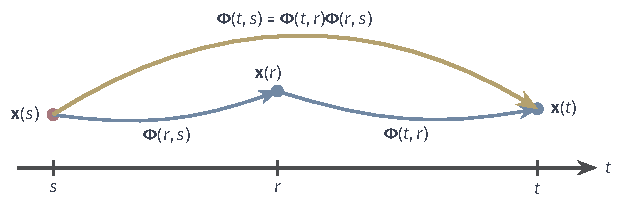
\includegraphics[width=105mm]{figures/06-differential-equations/01-ordinary-differential-equations/tikz/lde-transition-composition/figure.pdf}
  \caption{状态转移矩阵的复合。横轴是时间，红点是时刻$s$的状态，蓝点是其后的状态。两段蓝色箭头依次传播，黄色箭头直接传播，二者结果相同。矩阵乘积中晚的时刻写在左边。}
  \label{fig:lde-transition-composition}
\end{BookInlineFigure}

\begin{example}[一个可解的时变系统]
\label{ex:lde-time-varying}
取
\[
 \bm{A}(t)=\begin{bmatrix}0&t\\0&1\end{bmatrix},
\]
方程是$\dot{x}_1=tx_2$、$\dot{x}_2=x_2$。第二个方程先解出$x_2=\mathrm{e}^{t}x_2(0)$。代入第一个方程，再用分部积分，可知$t\mathrm{e}^{t}$的一个原函数是$(t-1)\mathrm{e}^{t}$。

于是$(1,0)^{\top}$和$((t-1)\mathrm{e}^{t},\mathrm{e}^{t})^{\top}$是两个解，把它们并排放置，得到基本解矩阵和它的逆：
\[
 \bm{X}(t)=\begin{bmatrix}1&(t-1)\mathrm{e}^{t}\\0&\mathrm{e}^{t}\end{bmatrix},\qquad
 \bm{X}(s)^{-1}=\begin{bmatrix}1&1-s\\0&\mathrm{e}^{-s}\end{bmatrix}.
\]
由式~\eqref{eq:lde-fundamental-to-transition}，
\[
 \bm{\Phi}(t,s)=\begin{bmatrix}1&(1-s)+(t-1)\mathrm{e}^{t-s}\\0&\mathrm{e}^{t-s}\end{bmatrix}.
\]
取$t=s$，右上角为$(1-s)+(s-1)=0$，符合$\bm{\Phi}(s,s)=\bm{I}$。再取时长都是$1$的两段：
\[
 \bm{\Phi}(1,0)=\begin{bmatrix}1&1\\0&\mathrm{e}\end{bmatrix},\qquad
 \bm{\Phi}(2,1)=\begin{bmatrix}1&\mathrm{e}\\0&\mathrm{e}\end{bmatrix}.
\]
它们不相等，说明传播同时依赖两个时刻，而不只依赖时长。它们的乘积是
\[
 \bm{\Phi}(2,1)\bm{\Phi}(1,0)=\begin{bmatrix}1&1+\mathrm{e}^2\\0&\mathrm{e}^2\end{bmatrix},
\]
这正是公式给出的$\bm{\Phi}(2,0)$，复合关系得到验证。
\end{example}

\paragraph{为什么不能积分后取指数}
现在可以检验开始时的想法了。对例~\ref{ex:lde-time-varying}的系数，从$0$积分得到
\[
 \bm{M}(t)=\int_0^t\bm{A}(r)\,\mathrm{d}r=\begin{bmatrix}0&t^2/2\\0&t\end{bmatrix}.
\]
固定$t$，写$\bm{M}=t\bm{B}$，其中$\bm{B}$满足$\bm{B}^2=\bm{B}$：
\[
 \bm{B}=\begin{bmatrix}0&t/2\\0&1\end{bmatrix}.
\]
于是级数中$\bm{B}^k$全部等于$\bm{B}$，求和得到
\[
 \mathrm{e}^{\bm{M}(t)}=\bm{I}+(\mathrm{e}^{t}-1)\bm{B}=\begin{bmatrix}1&(\mathrm{e}^{t}-1)t/2\\0&\mathrm{e}^{t}\end{bmatrix}.
\]

把它与$\bm{\Phi}(t,0)$的右上角比较：真解是$(t-1)\mathrm{e}^{t}+1$，直接取指数的结果是$(\mathrm{e}^{t}-1)t/2$。取$t=2$，前者是$\mathrm{e}^2+1\approx8.389$，后者是$\mathrm{e}^2-1\approx6.389$。图~\ref{fig:lde-noncommuting}中两条曲线随时间逐渐分开，绿点是对原方程作数值积分的结果，它落在蓝线上。

\begin{BookInlineFigure}
  \centering
  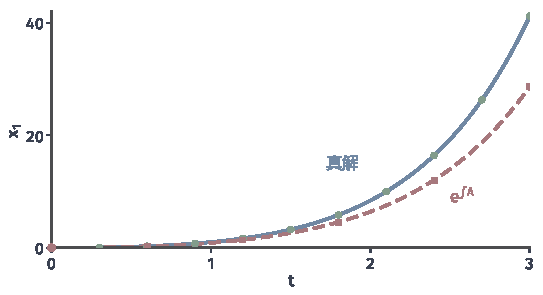
\includegraphics[width=92mm]{figures/06-differential-equations/01-ordinary-differential-equations/matplotlib/lde-noncommuting/figure.pdf}
  \caption{时变系统不能对系数积分后直接取指数。$\bm{A}(t)=\left[\begin{smallmatrix}0&t\\0&1\end{smallmatrix}\right]$，$\bm{x}(0)=(0,1)^{\top}$，图中是分量$x_1$。蓝线是真解$(t-1)\mathrm{e}^{t}+1$，绿点是步长$0.05$的四阶Runge--Kutta数值解；红色虚线是$\exp\int_0^t\bm{A}$给出的$(\mathrm{e}^{t}-1)t/2$，红色方点是对$\bm{M}(t)$直接计算矩阵指数的结果。}
  \label{fig:lde-noncommuting}
\end{BookInlineFigure}

失败的原因在求导。若想让$\mathrm{e}^{\bm{M}(t)}$满足方程，$\mathrm{e}^{\bm{M}}$的导数就要等于$\dot{\bm{M}}\mathrm{e}^{\bm{M}}$。看级数中的二次项：
\[
 \frac{\mathrm{d}}{\mathrm{d}t}\bm{M}^2=\dot{\bm{M}}\bm{M}+\bm{M}\dot{\bm{M}}.
\]
只有$\dot{\bm{M}}$与$\bm{M}$可交换时，它才等于$2\dot{\bm{M}}\bm{M}$。例中$\bm{A}(s)\bm{A}(t)=\bm{A}(s)$而$\bm{A}(t)\bm{A}(s)=\bm{A}(t)$，两个时刻的系数不可交换。

从传播的角度看更直观。$\exp\int\bm{A}$把各时刻的系数不分先后地加在一起，Peano--Baker级数却严格保留“晚的在左”的次序。图~\ref{fig:lde-switching-order}用两段常系数的切换说明次序的影响。设两段系数各作用单位时间：
\[
 \bm{A}_1=\begin{bmatrix}0&1\\0&0\end{bmatrix},\qquad \bm{A}_2=\begin{bmatrix}0&0\\1&0\end{bmatrix}.
\]
由$\bm{A}_1^2=\bm{A}_2^2=\bm{0}$，得$\mathrm{e}^{\bm{A}_i}=\bm{I}+\bm{A}_i$。

先用$\bm{A}_1$、后用$\bm{A}_2$的传播是
\[
 \mathrm{e}^{\bm{A}_2}\mathrm{e}^{\bm{A}_1}=\begin{bmatrix}1&1\\1&2\end{bmatrix}.
\]
次序反过来的传播是
\[
 \mathrm{e}^{\bm{A}_1}\mathrm{e}^{\bm{A}_2}=\begin{bmatrix}2&1\\1&1\end{bmatrix}.
\]
两种切换的系数积分都是$\bm{A}_1+\bm{A}_2$，而直接取指数得到
\[
 \mathrm{e}^{\bm{A}_1+\bm{A}_2}=\begin{bmatrix}\cosh1&\sinh1\\\sinh1&\cosh1\end{bmatrix},
\]
与两者都不同。这就像先向右剪切再向上剪切，与先向上剪切再向右剪切，结果是两个不同的平行四边形。

\begin{BookInlineFigure}
  \centering
  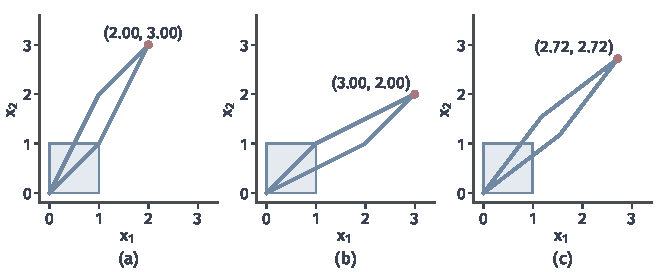
\includegraphics[width=112mm]{figures/06-differential-equations/01-ordinary-differential-equations/matplotlib/lde-switching-order/figure.pdf}
  \caption{切换次序影响结果，浅蓝方块是单位正方形，蓝线是它的像，红点是$(1,1)^{\top}$的像。(a)$\mathrm{e}^{\bm{A}_2}\mathrm{e}^{\bm{A}_1}$。(b)$\mathrm{e}^{\bm{A}_1}\mathrm{e}^{\bm{A}_2}$。(c)$\mathrm{e}^{\bm{A}_1+\bm{A}_2}$，它对应系数积分后直接取指数，不等于任何一种切换次序的实际传播。}
  \label{fig:lde-switching-order}
\end{BookInlineFigure}

\paragraph{可交换时的简化}
上面的分析也指出了简化公式成立的条件：让所有时刻的系数彼此可交换。

\begin{theorem}[可交换系数的状态转移矩阵]
\label{thm:lde-commuting}
设$\bm{A}$在$I$上连续，并且对任意$r,r'\in I$都有$\bm{A}(r)\bm{A}(r')=\bm{A}(r')\bm{A}(r)$。则
\begin{equation}
 \bm{\Phi}(t,s)=\exp\Bigl(\int_s^t\bm{A}(r)\,\mathrm{d}r\Bigr).
 \label{eq:lde-commuting}
\end{equation}
\end{theorem}

\begin{proof}
固定$s$，令$\bm{M}(t)=\int_s^t\bm{A}(r)\,\mathrm{d}r$。积分是Riemann和的极限，而每个Riemann和都与$\bm{A}(t)$可交换，所以$\bm{M}(t)\bm{A}(t)=\bm{A}(t)\bm{M}(t)$。

用乘积求导并归纳，$\frac{\mathrm{d}}{\mathrm{d}t}\bm{M}^k$是$k$项之和，每一项都把一个因子$\bm{M}$换成$\bm{A}(t)$。交换关系把$\bm{A}(t)$移到最左边，得到
\[
 \frac{\mathrm{d}}{\mathrm{d}t}\bm{M}^k=k\bm{A}(t)\bm{M}^{k-1}.
\]
逐项求导的级数在紧子区间上被$\lVert\bm{A}(t)\rVert_2\mathrm{e}^{\lVert\bm{M}(t)\rVert_2}$的同型优级数控制，所以求导合法，并且
\[
 \frac{\mathrm{d}}{\mathrm{d}t}\mathrm{e}^{\bm{M}(t)}=\bm{A}(t)\mathrm{e}^{\bm{M}(t)}.
\]
又有$\bm{M}(s)=\bm{0}$，由定理~\ref{thm:lde-transition-existence}的唯一性得到结论。
\end{proof}

定理的条件是充分条件。标量方程、对角系数和$\bm{A}(t)=a(t)\bm{B}$（$\bm{B}$为常矩阵）都满足它。最后一种情形有直观的含义：$a(t)$只决定沿$\bm{B}$的轨线走得多快，不改变轨线本身。例如$\bm{A}(t)=2t\bm{J}_0$时，式~\eqref{eq:lde-commuting}给出
\[
 \bm{\Phi}(t,0)=\mathrm{e}^{t^2\bm{J}_0}=\begin{bmatrix}\cos t^2&\sin t^2\\-\sin t^2&\cos t^2\end{bmatrix}.
\]
状态仍在圆周上转动，只是把时间换成了$t^2$。一般的时变系统没有这种闭式，$\bm{\Phi}$要靠数值方法求解，这由第~\ref{chap:ode-numerical-methods}章讨论。


\section{非齐次方程}
\label{sec:lde-inhomogeneous}

齐次传播建立之后，再加入外部输入。设$\bm{A}$、$\bm{g}$在区间$I$上连续，考虑
\begin{equation}
 \dot{\bm{x}}(t)=\bm{A}(t)\bm{x}(t)+\bm{g}(t),\qquad \bm{x}(t_0)=\bm{x}_0.
 \label{eq:lde-inhomogeneous}
\end{equation}
输入在每一时刻都推动状态，推动的效果又随齐次系统继续传播。怎样把这两件事合写成一个公式？

\paragraph{常数变易}
没有输入时，解是$\bm{\Phi}(t,t_0)\bm{c}$，其中$\bm{c}$是常向量，等于初始状态。输入不断改变状态，可以理解为“初始状态”这个系数在缓慢漂移。于是让$\bm{c}$依赖时间，设$\bm{x}(t)=\bm{\Phi}(t,t_0)\bm{c}(t)$，代入方程。

乘积求导时，$\partial_t\bm{\Phi}$产生的项恰好是$\bm{A}\bm{x}$，与方程右端抵消，只剩下
\[
 \bm{\Phi}(t,t_0)\dot{\bm{c}}(t)=\bm{g}(t).
\]
用$\bm{\Phi}(t,t_0)^{-1}=\bm{\Phi}(t_0,t)$乘两边，再由$\bm{c}(t_0)=\bm{x}_0$积分，得到
\[
 \bm{c}(t)=\bm{x}_0+\int_{t_0}^{t}\bm{\Phi}(t_0,s)\bm{g}(s)\,\mathrm{d}s.
\]

这一步也有含义：$\bm{\Phi}(t_0,s)\bm{g}(s)$把时刻$s$的输入折算回初始时刻。把$\bm{c}(t)$代回去，再用复合关系$\bm{\Phi}(t,t_0)\bm{\Phi}(t_0,s)=\bm{\Phi}(t,s)$，就得到下面的定理。

\begin{theorem}[常数变易公式]
\label{thm:lde-variation-of-constants}
设$\bm{A},\bm{g}$在$I$上连续，$t_0\in I$。初值问题~\eqref{eq:lde-inhomogeneous}在$I$上有唯一解，它是
\begin{equation}
 \bm{x}(t)=\bm{\Phi}(t,t_0)\bm{x}_0+\int_{t_0}^{t}\bm{\Phi}(t,s)\bm{g}(s)\,\mathrm{d}s.
 \label{eq:lde-variation-of-constants}
\end{equation}
常系数时$\bm{\Phi}(t,s)=\mathrm{e}^{(t-s)\bm{A}}$，公式成为
\begin{equation}
 \bm{x}(t)=\mathrm{e}^{(t-t_0)\bm{A}}\bm{x}_0+\int_{t_0}^{t}\mathrm{e}^{(t-s)\bm{A}}\bm{g}(s)\,\mathrm{d}s.
 \label{eq:lde-duhamel-constant}
\end{equation}
\end{theorem}

\begin{proof}
先检验式~\eqref{eq:lde-variation-of-constants}满足方程和初值。由复合关系，这个公式可以写成乘积$\bm{\Phi}(t,t_0)\bm{c}(t)$，其中$\bm{c}$如上。对乘积求导，得
\[
\begin{aligned}
 \dot{\bm{x}}(t)&=\bm{A}(t)\bm{\Phi}(t,t_0)\bm{c}(t)+\bm{\Phi}(t,t_0)\bm{\Phi}(t_0,t)\bm{g}(t)\\
 &=\bm{A}(t)\bm{x}(t)+\bm{g}(t).
\end{aligned}
\]
$t=t_0$时积分为零，$\bm{\Phi}(t_0,t_0)=\bm{I}$，所以$\bm{x}(t_0)=\bm{x}_0$。

再证唯一。两个解之差满足齐次方程，初值为零，由定理~\ref{thm:lde-transition-existence}恒为零。
\end{proof}

式~\eqref{eq:lde-variation-of-constants}称为\term{常数变易公式}（variation of constants formula），也称\term{Duhamel公式}（Duhamel formula）。若$\bm{g}$只在每个紧子区间上可积，公式不变，解是局部绝对连续的，方程几乎处处成立，这与定理~\ref{thm:lde-scalar-integrable}的论证相同。

\paragraph{初始状态响应与零初值响应}
公式的两项分别只含一种数据。第一项$\bm{\Phi}(t,t_0)\bm{x}_0$不依赖输入，称为\term{零输入响应}（zero-input response）。第二项不依赖初始状态，称为\term{零状态响应}（zero-state response）。

每一项都线性依赖自己的数据，总响应是两项之和。所以“响应”对数据对$(\bm{x}_0,\bm{g})$是线性的。常见的误解是说总响应关于输入线性：若$\bm{x}_0\neq\bm{0}$，把输入加倍并不会把总响应加倍，因为零输入响应没有变。

\begin{example}[阶跃输入的响应分解]
\label{ex:lde-step-response}
考虑$\ddot{x}+3\dot{x}+2x=1$，$x(0)=1$，$\dot{x}(0)=0$。状态形式用例~\ref{ex:lde-running-system}的矩阵，$\bm{g}=(0,1)^{\top}$，$\bm{x}_0=(1,0)^{\top}$。零输入响应的第一分量已经算过，是$2\mathrm{e}^{-t}-\mathrm{e}^{-2t}$。

零状态响应用到$\mathrm{e}^{r\bm{A}}$的第二列，它的第一分量是$\mathrm{e}^{-r}-\mathrm{e}^{-2r}$。在式~\eqref{eq:lde-duhamel-constant}中令$r=t-s$，积分变成
\[
 \int_0^t(\mathrm{e}^{-r}-\mathrm{e}^{-2r})\,\mathrm{d}r=\frac12-\mathrm{e}^{-t}+\frac12\mathrm{e}^{-2t}.
\]
两部分相加，得到总响应
\[
 x(t)=\frac12+\mathrm{e}^{-t}-\frac12\mathrm{e}^{-2t}.
\]
代回检验：$x(0)=1$，$\dot{x}=-\mathrm{e}^{-t}+\mathrm{e}^{-2t}$，所以$\dot{x}(0)=0$；再求$\ddot{x}=\mathrm{e}^{-t}-2\mathrm{e}^{-2t}$，并计算
\[
 \ddot{x}+3\dot{x}+2x=(1-3+2)\mathrm{e}^{-t}+(-2+3-1)\mathrm{e}^{-2t}+1=1.
\]
\end{example}

图~\ref{fig:lde-response-decomposition}中，黄线由初始状态决定，从$1$下降到$0$；紫线由输入决定，从$0$升到$1/2$。蓝线是二者之和。这个系统的状态最终停在$1/2$，只和输入有关，初值的痕迹全部由零输入响应带走。

\begin{BookInlineFigure}
  \centering
  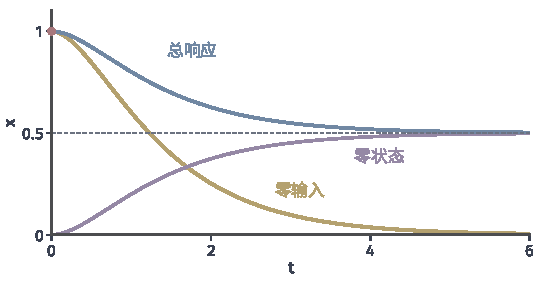
\includegraphics[width=92mm]{figures/06-differential-equations/01-ordinary-differential-equations/matplotlib/lde-response-decomposition/figure.pdf}
  \caption{响应的分解，方程$\ddot{x}+3\dot{x}+2x=1$，$x(0)=1$（红点），$\dot{x}(0)=0$。黄线是零输入响应，紫线是零状态响应，蓝线是总响应，灰色虚线是水平$1/2$。}
  \label{fig:lde-response-decomposition}
\end{BookInlineFigure}

\paragraph{受迫振动与共振}
荡秋千时，每次都在同一相位推一下，幅度就越来越大；推的节奏不对，推力再大也荡不高。把这个现象写成方程，就是无阻尼振子受周期外力：
\begin{equation}
 \ddot{x}+\omega_0^2x=\cos\omega t,\qquad x(0)=\dot{x}(0)=0,
 \label{eq:lde-forced-oscillator}
\end{equation}
其中$\omega_0>0$是固有频率，$\omega>0$是外力频率。

状态形式的系数矩阵如下，它满足$\bm{A}^2=-\omega_0^2\bm{I}$：
\[
 \bm{A}=\begin{bmatrix}0&1\\-\omega_0^2&0\end{bmatrix}.
\]
级数的偶次项和奇次项分别凑成余弦和正弦，得到
\[
 \mathrm{e}^{t\bm{A}}=\begin{bmatrix}\cos\omega_0t&\sin(\omega_0t)/\omega_0\\-\omega_0\sin\omega_0t&\cos\omega_0t\end{bmatrix}.
\]
输入是$(0,\cos\omega t)^{\top}$，所以式~\eqref{eq:lde-duhamel-constant}的第一分量是
\begin{equation}
 x(t)=\frac{1}{\omega_0}\int_0^t\sin\bigl(\omega_0(t-s)\bigr)\cos(\omega s)\,\mathrm{d}s.
 \label{eq:lde-forced-integral}
\end{equation}

用积化和差把被积函数拆开：
\[
 \begin{aligned}
 \sin(\omega_0(t-s))\cos\omega s={}&\tfrac12\sin\bigl(\omega_0t-(\omega_0-\omega)s\bigr)\\
 &+\tfrac12\sin\bigl(\omega_0t-(\omega_0+\omega)s\bigr).
 \end{aligned}
\]
当$\omega\neq\omega_0$时，两项都对$s$积分，第一项给出$(\cos\omega t-\cos\omega_0t)/(\omega_0-\omega)$，第二项给出$(\cos\omega t-\cos\omega_0t)/(\omega_0+\omega)$。代入式~\eqref{eq:lde-forced-integral}并通分，
\begin{equation}
 x(t)=\frac{\cos\omega t-\cos\omega_0t}{\omega_0^2-\omega^2},\qquad \omega\neq\omega_0.
 \label{eq:lde-off-resonance}
\end{equation}
这个解有界，幅度不超过$2/\lvert\omega_0^2-\omega^2\rvert$。$\omega$接近$\omega_0$时，两个余弦的频率相近，交替增强与抵消，形成缓慢起伏的\term{拍}（beat）。

当$\omega=\omega_0$时，第一项是常数$\tfrac12\sin\omega_0t$，它对$s$积分得到$\tfrac12t\sin\omega_0t$。第二项在$[0,t]$上的积分为
\[
 \frac12\Bigl[\frac{\cos(\omega_0t-2\omega_0s)}{2\omega_0}\Bigr]_{s=0}^{s=t}=0.
\]
于是
\begin{equation}
 x(t)=\frac{t\sin\omega_0t}{2\omega_0},\qquad \omega=\omega_0.
 \label{eq:lde-resonance}
\end{equation}
代回检验，取$\omega_0=1$，$x=\tfrac12t\sin t$。两次求导得到
\[
 \dot{x}=\frac{\sin t+t\cos t}{2},\qquad \ddot{x}=\cos t-\frac{t\sin t}{2}.
\]
所以$\ddot{x}+x=\cos t$，并且$x(0)=\dot{x}(0)=0$。

这种振幅按$t$线性增长的现象称为\term{共振}（resonance）。图~\ref{fig:lde-resonance}取$\omega_0=1$比较三种外力频率。外力大小完全相同，差别只在频率：$\omega=2$时响应很小，$\omega=1.2$时出现拍，$\omega=1$时振幅沿紫色虚线$\pm t/2$增长。

\begin{BookInlineFigure}
  \centering
  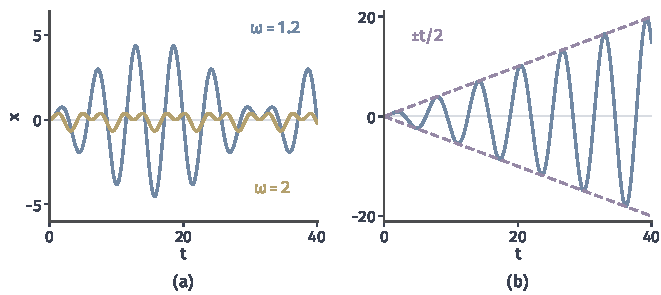
\includegraphics[width=112mm]{figures/06-differential-equations/01-ordinary-differential-equations/matplotlib/lde-resonance/figure.pdf}
  \caption{方程~\eqref{eq:lde-forced-oscillator}取$\omega_0=1$的零初值响应。(a)$\omega=2$（黄）的响应有界，$\omega=1.2$（蓝）出现拍。(b)$\omega=1$时发生共振，响应$t\sin t/2$的振幅沿紫色虚线$\pm t/2$线性增长。}
  \label{fig:lde-resonance}
\end{BookInlineFigure}

共振的原因要看积分~\eqref{eq:lde-forced-integral}的被积函数。$\sin(\omega_0(t-s))$是时刻$s$的单位冲击到时刻$t$还留下的响应，$\cos\omega s$是那一刻的外力。图~\ref{fig:lde-resonance-integrand}固定$t=4.5\pi$，画出被积函数对$s$的形状。

$\omega=1$时被积函数不变号，每一时刻的贡献都同向累加，面积是$t/2\approx7.07$。$\omega=2$时正负面积大部分抵消，只剩$1/3$。所以共振并不是输入太大，而是输入与齐次模式同频，各时刻留下的响应到达同一时刻时相位一致。

这与第~\ref{sec:lde-constant}节的多项式因子是同一个机制：Jordan链上一级的输出含有下一级自身的模式，这里外力含有振子自身的模式，于是都多出一个因子$t$。无阻尼模型的振幅没有上界。若有阻尼，齐次模式按指数衰减，早期输入留下的响应会逐渐消失，累积不再无限制地增长。

\begin{BookInlineFigure}
  \centering
  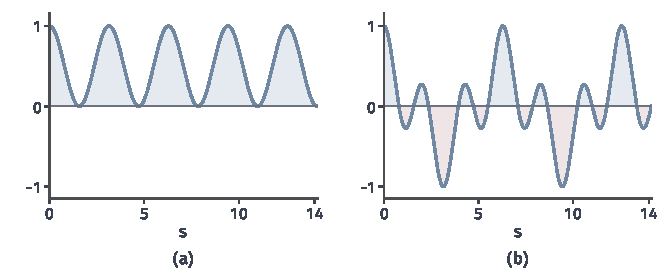
\includegraphics[width=112mm]{figures/06-differential-equations/01-ordinary-differential-equations/matplotlib/lde-resonance-integrand/figure.pdf}
  \caption{共振的累积机制。式~\eqref{eq:lde-forced-integral}取$\omega_0=1$、$t=4.5\pi$时的被积函数$\sin(t-s)\cos\omega s$，浅蓝为正面积，浅红为负面积。(a)$\omega=1$，被积函数不变号，积分约为$7.07$。(b)$\omega=2$，正负抵消，积分为$1/3$。}
  \label{fig:lde-resonance-integrand}
\end{BookInlineFigure}


\section{因果Green函数}
\label{sec:lde-green}

常数变易公式中，积分号里的$\bm{\Phi}(t,s)$单独拿出来是什么意思？做一个思想实验：系统原本静止，在时刻$s$突然敲它一下，随后观察它的响应。

\paragraph{窄脉冲的极限}
“敲一下”可以用一个窄而高的矩形输入来描述。取单位面积的脉冲：在$[s,s+\varepsilon)$上输入为$\varepsilon^{-1}\bm{e}_j$，其余时刻为零，$\bm{e}_j$是第$j$个坐标方向。以零初值代入式~\eqref{eq:lde-variation-of-constants}。输入开始前响应为零，输入结束后，当$t\geq s+\varepsilon$时，
\[
 \bm{x}_{\varepsilon}(t)=\frac{1}{\varepsilon}\int_s^{s+\varepsilon}\bm{\Phi}(t,r)\bm{e}_j\,\mathrm{d}r.
\]

由定理~\ref{thm:lde-transition-properties}的(3)，$\bm{\Phi}(t,r)$对$r$连续，所以$\varepsilon\to0$时积分平均趋于$r=s$处的值。对每个$t>s$，
\begin{equation}
 \lim_{\varepsilon\to0^+}\bm{x}_{\varepsilon}(t)=\bm{\Phi}(t,s)\bm{e}_j,
 \label{eq:lde-pulse-limit}
\end{equation}
而$t<s$时响应恒为零。$\bm{\Phi}(t,s)$的第$j$列就是这样一种响应：在时刻$s$沿第$j$个方向敲一下，系统在时刻$t$的状态。

\begin{definition}[因果Green函数]
\label{def:lde-causal-green}
对$t,s\in I$，线性系统$\dot{\bm{x}}=\bm{A}(t)\bm{x}+\bm{g}$的\term{因果Green函数}（causal Green's function）定义为
\begin{equation}
 \bm{G}(t,s)=\bm{\Phi}(t,s)\mathbb{I}_{[s,\infty)}(t),
 \label{eq:lde-causal-green}
\end{equation}
其中$\mathbb{I}_{[s,\infty)}$是区间$[s,\infty)$的示性函数。$\bm{G}(t,s)$在$t<s$时为零。
\end{definition}

有了$\bm{G}$，零状态响应（记为$\bm{x}_{\mathrm{zs}}$）可以写成对整段时间的积分。设$\bm{g}$在$[t_0,T]$上连续，$t\in[t_0,T]$，由$\bm{G}$在$s>t$时为零，得
\begin{equation}
 \bm{x}_{\mathrm{zs}}(t)=\int_{t_0}^{T}\bm{G}(t,s)\bm{g}(s)\,\mathrm{d}s.
 \label{eq:lde-green-solution}
\end{equation}
积分虽然延伸到$T$，实际只用到$s\leq t$的输入。这就是“因果”的含义：未来的输入不影响现在的状态。

$\bm{G}$在对角线$t=s$处有跳变。从$t<s$一侧的$\bm{0}$跳到$t>s$一侧的$\bm{I}$，所以
\begin{equation}
 \bm{G}(s^+,s)-\bm{G}(s^-,s)=\bm{I}.
 \label{eq:lde-green-jump}
\end{equation}
$t\neq s$时，$\bm{G}$对$t$满足齐次方程。工程和物理中常把这两条性质合写成
\[
 (\partial_t-\bm{A}(t))\bm{G}(t,s)=\delta(t-s)\bm{I}.
\]
这里的$\delta$不是普通函数，这个写法只是式~\eqref{eq:lde-pulse-limit}和跳变条件~\eqref{eq:lde-green-jump}的简写。

\paragraph{标量例子与脉冲响应}
常系数时$\bm{G}$只依赖时间差，$\bm{G}(t,s)=\bm{H}(t-s)$，其中
\begin{equation}
 \bm{H}(t)=\mathrm{e}^{t\bm{A}}\mathbb{I}_{[0,\infty)}(t).
 \label{eq:lde-constant-green}
\end{equation}
取$t_0=0$，零状态响应就是一个卷积：
\begin{equation}
 \bm{x}_{\mathrm{zs}}(t)=\int_0^t\bm{H}(t-s)\bm{g}(s)\,\mathrm{d}s.
 \label{eq:lde-convolution-response}
\end{equation}
时变系统没有这个简化。例如$\dot{x}=-2tx+g$的Green函数是
\[
 G(t,s)=\mathrm{e}^{s^2-t^2}\mathbb{I}_{[s,\infty)}(t),
\]
它依赖$s$和$t$本身，而不只是$t-s$。

高阶方程$p(\mathrm{D})x=g$由式~\eqref{eq:lde-companion}进入状态形式，输入只作用在最后一个分量上。单位脉冲让状态跳变$\bm{e}_n$：只有最高一阶导数$\mathrm{D}^{n-1}x$跳变$1$，$x$及更低阶的导数仍然连续。所以\term{脉冲响应}（impulse response）$w$是齐次方程在下列初值下的解：
\begin{equation}
 p(\mathrm{D})w=0,\qquad \mathrm{D}^{j}w(0)=0\ (j\leq n-2),\quad \mathrm{D}^{n-1}w(0)=1.
 \label{eq:lde-impulse-response}
\end{equation}
相应的零状态响应是$x(t)=\int_0^tw(t-s)g(s)\,\mathrm{d}s$。

对$\ddot{x}+3\dot{x}+2x=g$，$w$是$\mathrm{e}^{-t}$和$\mathrm{e}^{-2t}$的组合。由$w(0)=0$、$\dot{w}(0)=1$解出
\[
 w(t)=\mathrm{e}^{-t}-\mathrm{e}^{-2t},\qquad t\geq0.
\]
它就是例~\ref{ex:lde-step-response}中积分的被积函数，$g\equiv1$的响应正是$\int_0^tw(r)\,\mathrm{d}r$。图~\ref{fig:lde-pulse-limit}验证了脉冲极限：宽度$\varepsilon$减小时，矩形输入越来越高，响应却收敛到同一条曲线$w$。

\begin{BookInlineFigure}
  \centering
  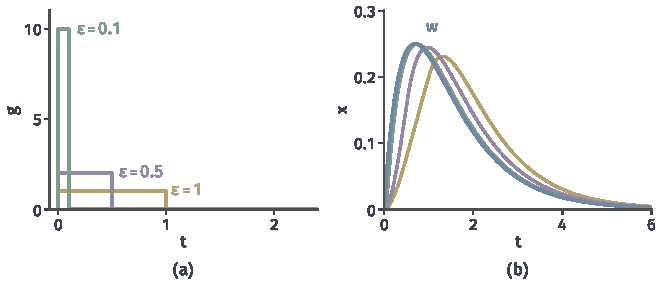
\includegraphics[width=112mm]{figures/06-differential-equations/01-ordinary-differential-equations/matplotlib/lde-pulse-limit/figure.pdf}
  \caption{窄脉冲的响应趋于脉冲响应，方程$\ddot{x}+3\dot{x}+2x=g$，零初值。(a)单位面积的矩形输入，宽度$\varepsilon=1,0.5,0.1$。(b)相同颜色的线是对应的精确响应，蓝线是脉冲响应$w=\mathrm{e}^{-t}-\mathrm{e}^{-2t}$。}
  \label{fig:lde-pulse-limit}
\end{BookInlineFigure}

\paragraph{输入是脉冲的叠加}
叠加原理让这个思想实验变成计算方法。把输入切成许多细长的矩形，每个矩形近似一次脉冲，响应是它们各自响应的总和；矩形变窄时，这个和就成为积分~\eqref{eq:lde-green-solution}。

取$\dot{x}=-x+g$，$g(t)=1+\cos t$，$x(0)=0$，此时$G(t,s)$在$t\geq s$时等于$\mathrm{e}^{-(t-s)}$。直接积分时用到
\[
 \int_0^t\mathrm{e}^{-(t-s)}\cos s\,\mathrm{d}s=\frac{\cos t+\sin t-\mathrm{e}^{-t}}{2},
\]
于是
\[
 x(t)=1+\frac{\cos t+\sin t}{2}-\frac32\mathrm{e}^{-t}.
\]

图~\ref{fig:lde-impulse-superposition}把$[0,6]$切成宽$0.5$的矩形。(b)中每条黄线是一个矩形的响应：输入期间上升，输入结束后按$\mathrm{e}^{-t}$衰减。它们的和（绿线）已经很接近精确解（蓝线），矩形取得更窄时差别还会减小。

\begin{BookInlineFigure}
  \centering
  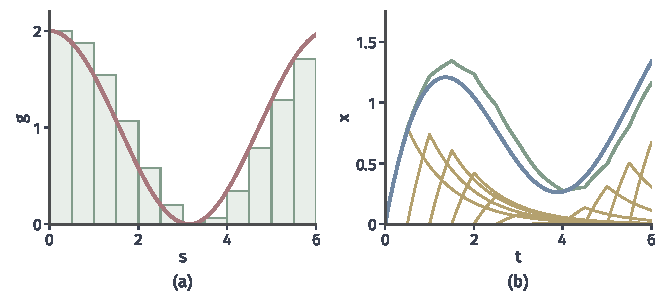
\includegraphics[width=112mm]{figures/06-differential-equations/01-ordinary-differential-equations/matplotlib/lde-impulse-superposition/figure.pdf}
  \caption{输入响应是脉冲响应的叠加，方程$\dot{x}=-x+g$，$x(0)=0$。(a)红线是输入$g=1+\cos s$，绿色矩形是宽$0.5$的分段常值近似，高度取矩形左端的$g$值。(b)黄线是单个矩形输入的响应，绿线是它们的和，蓝线是精确解。}
  \label{fig:lde-impulse-superposition}
\end{BookInlineFigure}

\paragraph{把算子看成下三角矩阵}
把函数看成无限维向量，可以换一个角度理解$\bm{G}$。在等距网格$t_k=t_0+kh$上，式~\eqref{eq:lde-green-solution}近似为一个矩阵乘向量：
\[
 x(t_i)\approx\sum_{j<i}hG(t_i,t_j)g(t_j).
\]
矩阵的第$(i,j)$元是$hG(t_i,t_j)$。第$j$列是在时刻$t_j$敲一下之后的响应序列，第$i$行说明时刻$t_i$的状态怎样加权历史上的输入。

$G(t_i,t_j)$在$j>i$时为零，这个矩阵是下三角的，所以因果性就是下三角结构。图~\ref{fig:lde-green-heatmap}(a)画出$\dot{x}=-x+g$的$G(t,s)$，只有对角线上方有值。类比的限度在于对角线：矩阵元是有限数，而$G$在对角线上的跳变对应着连续问题中$\delta$的位置，它不是任何矩阵元能单独表示的。

同样叫Green函数，边值问题的情形却不同。图~\ref{fig:lde-green-heatmap}(b)是$-\mathrm{d}^2u/\mathrm{d}x^2=f$、$u(0)=u(1)=0$的积分核$\min(x,s)(1-\max(x,s))$，它在对角线两侧都不为零。空间中的边界条件同时从两端约束解，一点的源影响所有位置，没有“先后”可言。这种边值Green函数由第~\ref{chap:elliptic-equations}章介绍。

\begin{BookInlineFigure}
  \centering
  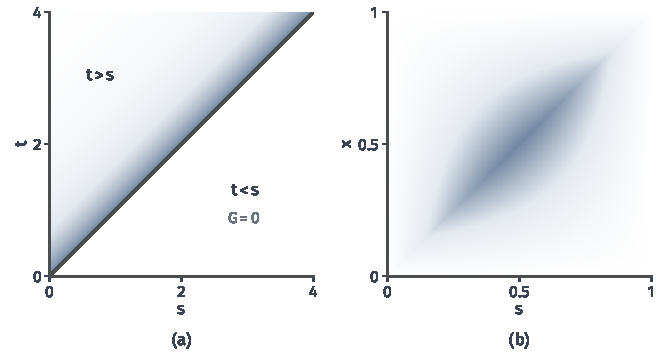
\includegraphics[width=112mm]{figures/06-differential-equations/01-ordinary-differential-equations/matplotlib/lde-green-heatmap/figure.pdf}
  \caption{因果Green函数与边值积分核的对比，颜色越深表示数值越大。(a)$G(t,s)=\mathrm{e}^{-(t-s)}\mathbb{I}_{[s,\infty)}(t)$，深灰线是对角线$t=s$，其下方$G$为零，体现因果性。(b)两点边值问题的核$\min(x,s)(1-\max(x,s))$，对角线两侧都不为零。}
  \label{fig:lde-green-heatmap}
\end{BookInlineFigure}


\section{Laplace变换求解}
\label{sec:lde-laplace}

常系数方程的公式已经齐备，但计算$\mathrm{e}^{t\bm{A}}$和卷积积分有时并不轻松。另一条路线是把求导变成乘法，把初值自动放进代数方程，再把结果翻译回时间域。这条路线要回答三件事：变换何时有定义，初值怎样进入，反过来的翻译是否唯一？

\paragraph{用指数权给函数“称重”}
考虑积分$\int_0^{\infty}\mathrm{e}^{-zt}f(t)\,\mathrm{d}t$。$\mathrm{e}^{-zt}$是一个衰减的权，$z$的实部越大，权衰减得越快，增长的函数也能被压住。图~\ref{fig:lde-laplace-weight}取$f=\mathrm{e}^{t}$：$z=0.5$时乘积仍在增长，$z=1$时是常数，只有$z=2$时乘积衰减，积分收敛。

把$z$取遍一个半平面，就得到一族读数，它们记录了$f$的全部信息。与Fourier变换相比，这里只积分$t\geq0$，并带有衰减权，所以允许指数增长的函数；当$z$在虚轴上时，它就是$f\mathbb{I}_{[0,\infty)}$的Fourier变换。后者的性质可参考\BookChapterRef{chap:fourier-transform}{卷四第14章“Fourier变换”}。

\begin{BookInlineFigure}
  \centering
  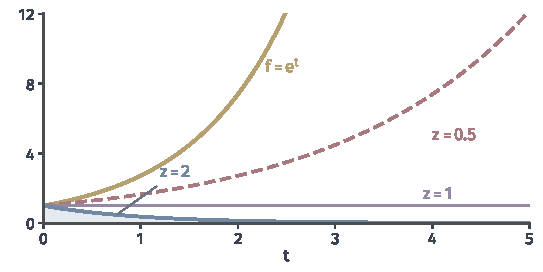
\includegraphics[width=92mm]{figures/06-differential-equations/01-ordinary-differential-equations/matplotlib/lde-laplace-weight/figure.pdf}
  \caption{指数权压住增长。黄线是$f=\mathrm{e}^{t}$，其余曲线是乘积$\mathrm{e}^{-zt}f(t)$：红色虚线$z=0.5$仍增长，紫线$z=1$恒为$1$，蓝线$z=2$衰减，浅蓝是收敛积分的面积$1$。}
  \label{fig:lde-laplace-weight}
\end{BookInlineFigure}

\begin{definition}[单边Laplace变换]
\label{def:lde-laplace}
设$f:[0,\infty)\to\mathbb{C}$在每个有界区间上分段连续（有限个间断点，左右极限都有限），且存在常数$M\geq0$和$c\in\mathbb{R}$使$\lvert f(t)\rvert\leq M\mathrm{e}^{ct}$对所有$t\geq0$成立，就称$f$是\term{指数阶函数}（function of exponential order）。对$\operatorname{Re}z>c$，定义$f$的\term{单边Laplace变换}（unilateral Laplace transform）
\begin{equation}
 \hat{f}(z)=\mathcal{L}[f](z)=\int_0^{\infty}\mathrm{e}^{-zt}f(t)\,\mathrm{d}t.
 \label{eq:lde-laplace}
\end{equation}
\end{definition}

记$\sigma=\operatorname{Re}z$。$\sigma>c$时被积函数的模不超过$M\mathrm{e}^{-(\sigma-c)t}$，所以积分绝对收敛，并且$\lvert\hat{f}(z)\rvert\leq M/(\sigma-c)$。不是每个函数都有变换：$\mathrm{e}^{t^2}$增长得比任何指数都快，对任何$z$积分都发散。

\paragraph{常用变换对}
直接积分可得$\mathcal{L}[\mathrm{e}^{at}](z)=1/(z-a)$，收敛条件是$\operatorname{Re}z>\operatorname{Re}a$。令$a$取$\pm\mathrm{i}\beta$再线性组合，得到正弦和余弦；对$a$逐次求导，得到$t^k\mathrm{e}^{at}$。表~\ref{tab:lde-laplace-pairs}列出本节用到的结果。

\begin{BookInlineTable}
  \centering
  \caption{常用的单边Laplace变换对，$k$为非负整数，$a\in\mathbb{C}$，$\beta,\tau$为实数，$\tau\geq0$。}
  \label{tab:lde-laplace-pairs}
  \begin{tabular}{lll}
    \toprule
    $f(t)$ & $\hat{f}(z)$ & 收敛范围\\
    \midrule
    $\mathrm{e}^{at}$ & $1/(z-a)$ & $\operatorname{Re}z>\operatorname{Re}a$\\
    $t^k\mathrm{e}^{at}$ & $k!/(z-a)^{k+1}$ & $\operatorname{Re}z>\operatorname{Re}a$\\
    $\cos\beta t$ & $z/(z^2+\beta^2)$ & $\operatorname{Re}z>0$\\
    $\sin\beta t$ & $\beta/(z^2+\beta^2)$ & $\operatorname{Re}z>0$\\
    $\mathrm{e}^{at}f(t)$ & $\hat{f}(z-a)$ & $\operatorname{Re}z>c+\operatorname{Re}a$\\
    $f(t-\tau)\mathbb{I}_{[\tau,\infty)}(t)$ & $\mathrm{e}^{-\tau z}\hat{f}(z)$ & $\operatorname{Re}z>c$\\
    \bottomrule
  \end{tabular}
\end{BookInlineTable}

\paragraph{导数公式：初值从这里进入}
方程能被化成代数式，靠的是下面的公式。它也说明了连续性为什么不能省略。

\begin{theorem}[导数的Laplace变换]
\label{thm:lde-laplace-derivative}
设$f$在$[0,\infty)$上连续，分段连续可微，$\dot{f}$是指数阶函数，$\lvert\dot{f}(t)\rvert\leq M\mathrm{e}^{ct}$，其中$c>0$。则$f$也是指数阶函数，并且对$\operatorname{Re}z>c$，
\begin{equation}
 \mathcal{L}[\dot{f}](z)=z\hat{f}(z)-f(0).
 \label{eq:lde-laplace-derivative}
\end{equation}
\end{theorem}

\begin{proof}
由$f(t)=f(0)+\int_0^t\dot{f}$，得到
\[
 \lvert f(t)\rvert\leq\lvert f(0)\rvert+\frac{M}{c}\mathrm{e}^{ct},
\]
所以$f$是指数阶函数。

设$\dot{f}$的间断点为$t_1<t_2<\cdots$。在每一段上分部积分，并把$[0,T]$上的各段相加。$f$连续，所以内部接缝处的边界项两两抵消，只剩两端：
\[
 \int_0^T\mathrm{e}^{-zt}\dot{f}(t)\,\mathrm{d}t=\mathrm{e}^{-zT}f(T)-f(0)+z\int_0^T\mathrm{e}^{-zt}f(t)\,\mathrm{d}t.
\]
$\operatorname{Re}z>c$时，$\lvert\mathrm{e}^{-zT}f(T)\rvert\to0$。令$T\to\infty$就得到结论。
\end{proof}

连续性用在边界项的抵消上。若$f$有跳变，比如$f=\mathbb{I}_{[1,\infty)}$，则$\dot{f}$几乎处处为零，$\mathcal{L}[\dot{f}]=0$；而$z\hat{f}(z)-f(0)=\mathrm{e}^{-z}\neq0$，差额恰好是跳变项。

把公式用两次，得到二阶导数的变换：
\begin{equation}
 \mathcal{L}[\ddot{f}](z)=z^2\hat{f}(z)-zf(0)-\dot{f}(0).
 \label{eq:lde-laplace-second}
\end{equation}
这里要求$f$和$\dot{f}$连续。初值以多项式的形式出现在右端，所以不需要先求通解、再定常数。

\paragraph{卷积与唯一性}
式~\eqref{eq:lde-convolution-response}的卷积也有简单的像。对$[0,\infty)$上的函数，记$(f*g)(t)=\int_0^tf(t-s)g(s)\,\mathrm{d}s$。

\begin{theorem}[卷积定理]
\label{thm:lde-laplace-convolution}
设$f,g$是指数阶函数，相应的增长指数都不超过$c$。则$f*g$连续并且是指数阶函数，对$\operatorname{Re}z>c$有
\begin{equation}
 \mathcal{L}[f*g](z)=\hat{f}(z)\hat{g}(z).
 \label{eq:lde-laplace-convolution}
\end{equation}
\end{theorem}

\begin{proof}
由$\lvert f\rvert\leq M_1\mathrm{e}^{ct}$和$\lvert g\rvert\leq M_2\mathrm{e}^{ct}$，得$\lvert(f*g)(t)\rvert\leq M_1M_2t\mathrm{e}^{ct}$，它不超过常数乘$\mathrm{e}^{c't}$（任取$c'>c$）。连续性可由控制收敛定理得到。

设$\sigma=\operatorname{Re}z>c$。二重积分
\[
 \int_0^{\infty}\!\!\int_0^t\lvert\mathrm{e}^{-zt}f(t-s)g(s)\rvert\,\mathrm{d}s\,\mathrm{d}t\leq\frac{M_1M_2}{(\sigma-c)^2}
\]
有限：非负被积函数可以先对$t$积分，令$r=t-s$就得到右端的界。所以可用Fubini定理交换积分次序，同样令$r=t-s$：
\[
 \int_0^{\infty}\!\!\int_s^{\infty}\mathrm{e}^{-zt}f(t-s)g(s)\,\mathrm{d}t\,\mathrm{d}s=\int_0^{\infty}\mathrm{e}^{-zs}g(s)\,\mathrm{d}s\int_0^{\infty}\mathrm{e}^{-zr}f(r)\,\mathrm{d}r.
\]
右端正是$\hat{f}(z)\hat{g}(z)$。
\end{proof}

从像函数翻译回时间函数，要先知道翻译是唯一的。函数在个别点上的取值不影响积分，所以唯一性只能精确到这些点。

\begin{theorem}[Laplace变换的唯一性]
\label{thm:lde-laplace-uniqueness}
设$f_1,f_2$是指数阶函数，并且存在实数$b$，使$\hat{f}_1(z)=\hat{f}_2(z)$对所有$z>b$的实数成立。则在$f_1$和$f_2$的每个公共连续点上都有$f_1=f_2$。
\end{theorem}

\begin{proof}
令$f=f_1-f_2$，取整数$k>\max(b,c)$，其中$c$使$\lvert f\rvert\leq M\mathrm{e}^{ct}$成立。作代换$u=\mathrm{e}^{-t}$，令$\varphi(u)=u^{k}f(-\ln u)$，$u\in(0,1]$。由$\lvert\varphi(u)\rvert\leq Mu^{k-c}$，$\varphi$在$(0,1]$上有界。对$m=0,1,2,\ldots$，
\[
 0=\hat{f}(k+1+m)=\int_0^{\infty}\mathrm{e}^{-(k+1+m)t}f(t)\,\mathrm{d}t=\int_0^1u^{m}\varphi(u)\,\mathrm{d}u.
\]

所以$\varphi$与每个多项式的乘积积分为零。给定$\eta>0$，取$[0,1]$上的连续函数$\psi$使$\int_0^1\lvert\varphi-\psi\rvert\leq\eta$，由Weierstrass逼近定理再取多项式$q$，使$\sup\lvert\psi-q\rvert\leq\eta$，记$B=\sup\lvert\varphi\rvert$。于是
\[
 \int_0^1\lvert\varphi\rvert^2=\int_0^1\bar{\varphi}(\varphi-\psi)+\int_0^1\bar{\varphi}(\psi-q)+\int_0^1\bar{\varphi}q.
\]
最后一项是$\int_0^1\varphi\bar{q}$的共轭，等于零，前两项各不超过$B\eta$，所以$\int_0^1\lvert\varphi\rvert^2\leq2B\eta$。$\eta$任意，得$\int_0^1\lvert\varphi\rvert^2=0$。分段连续函数平方积分为零，就在其每个连续点上为零。
\end{proof}

证明中的多项式逼近定理可参考\BookChapterRef{chap:function-approximation}{卷四第20章“函数逼近”}。定理告诉我们，只要在表中找到一个时间函数，它的变换等于所求的像函数，这个函数就是答案。一般的反演积分公式需要复变函数，本节的有理函数都用部分分式和查表处理，不必用到它。

\paragraph{求解的三步}
常系数方程的求解分三步。第一步，对方程两边作变换，用式~\eqref{eq:lde-laplace-derivative}和式~\eqref{eq:lde-laplace-second}代入初值，得到关于$\hat{x}$的代数方程。第二步，解出$\hat{x}$，它通常是有理函数。第三步，把$\hat{x}$拆成部分分式，查表得到$x$，再代回原问题检验。

\begin{example}[带初值的阶跃响应]
\label{ex:lde-laplace-step}
求解例~\ref{ex:lde-step-response}的问题$\ddot{x}+3\dot{x}+2x=1$，$x(0)=1$，$\dot{x}(0)=0$。作变换，右端的像是$1/z$，左端由式~\eqref{eq:lde-laplace-second}和式~\eqref{eq:lde-laplace-derivative}得到
\[
 (z^2\hat{x}-z)+3(z\hat{x}-1)+2\hat{x}=\frac1z.
\]
合并含$\hat{x}$的项，并解出
\[
 \hat{x}(z)=\frac{z^2+3z+1}{z(z+1)(z+2)}.
\]
三个极点都是单极点。对单极点$p$，部分分式的系数是把因子$(z-p)$约去后在$z=p$处取值，于是
\[
 \hat{x}(z)=\frac{1/2}{z}+\frac{1}{z+1}-\frac{1/2}{z+2}.
\]
由表~\ref{tab:lde-laplace-pairs}，
\[
 x(t)=\frac12+\mathrm{e}^{-t}-\frac12\mathrm{e}^{-2t},\qquad t\geq0.
\]
这与例~\ref{ex:lde-step-response}的结果一致，那里已经代回方程检验过。最右边的极点是$0$，所以像函数在$\operatorname{Re}z>0$上收敛。
\end{example}

收敛范围与极点的位置直接相关：解的增长指数由最右边的极点决定，收敛半平面从那里开始，图~\ref{fig:lde-laplace-region}给出三个例子。极点的虚部对应振荡，重数对应多项式因子，这与第~\ref{sec:lde-constant}节的特征根完全对应。

\begin{BookInlineFigure}
  \centering
  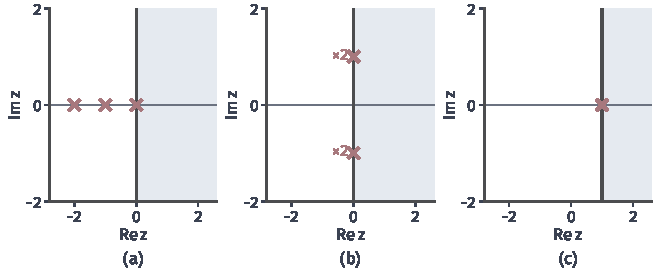
\includegraphics[width=112mm]{figures/06-differential-equations/01-ordinary-differential-equations/matplotlib/lde-laplace-region/figure.pdf}
  \caption{像函数的极点（红叉）与收敛半平面（浅蓝，边界为深灰竖线）。(a)例~\ref{ex:lde-laplace-step}的极点$0,-1,-2$。(b)共振例的二重极点$\pm\mathrm{i}$。(c)$\mathrm{e}^{t}$的极点$1$，收敛范围是$\operatorname{Re}z>1$。}
  \label{fig:lde-laplace-region}
\end{BookInlineFigure}

\paragraph{复极点、重极点与共振}
复极点常用配方处理。对$\ddot{x}+2\dot{x}+5x=0$，$x(0)=1$，$\dot{x}(0)=0$，同样作变换解出$\hat{x}=(z+2)/(z^2+2z+5)$。分母配方为$(z+1)^2+4$，分子写成$(z+1)+1$，于是
\[
 \hat{x}(z)=\frac{z+1}{(z+1)^2+4}+\frac12\cdot\frac{2}{(z+1)^2+4}.
\]
用表中的平移规则和正弦、余弦的变换，得到$x(t)=\mathrm{e}^{-t}(\cos2t+\frac12\sin2t)$，与第~\ref{sec:lde-high-order}节的结果相同。

重极点对应输入与齐次模式的配合。取$\ddot{x}+2\dot{x}+x=\mathrm{e}^{-t}$，零初值。特征根$-1$是二重的，输入又含有同一模式，像函数的极点升到三重：
\[
 \hat{x}(z)=\frac{1}{(z+1)^3}.
\]
由表得$x(t)=\frac12t^2\mathrm{e}^{-t}$。代回检验，
\[
 \dot{x}=\Bigl(t-\frac{t^2}{2}\Bigr)\mathrm{e}^{-t},\qquad
 \ddot{x}=\Bigl(1-2t+\frac{t^2}{2}\Bigr)\mathrm{e}^{-t}.
\]
于是$\ddot{x}+2\dot{x}+x=\mathrm{e}^{-t}$，且$x(0)=\dot{x}(0)=0$。

卷积定理把这一节和常数变易公式联系起来。式~\eqref{eq:lde-forced-oscillator}取$\omega_0=\omega=1$，作变换得
\[
 \hat{x}(z)=\frac{z}{(z^2+1)^2}=\frac{1}{z^2+1}\cdot\frac{z}{z^2+1}.
\]
两个因子分别是$\sin t$和$\cos t$的像，乘积对应卷积$\int_0^t\sin(t-s)\cos s\,\mathrm{d}s$，这正是积分~\eqref{eq:lde-forced-integral}。另一方面，对表中$\mathcal{L}[\sin t](z)=1/(z^2+1)$关于$z$求导，可得$\mathcal{L}[t\sin t](z)=2z/(z^2+1)^2$，于是$x(t)=\tfrac12t\sin t$，与式~\eqref{eq:lde-resonance}相同。二重极点$\pm\mathrm{i}$就是频率上的共振。

\paragraph{分段输入}
延迟规则让分段输入也能一次写出。取$\dot{x}=-x+g$，$x(0)=0$，$g$在$[0,1)$上为$1$，其余时刻为$0$。写$g=\mathbb{I}_{[0,\infty)}-\mathbb{I}_{[1,\infty)}$，得$\hat{g}=(1-\mathrm{e}^{-z})/z$，于是
\[
 \hat{x}(z)=(1-\mathrm{e}^{-z})\Bigl(\frac1z-\frac{1}{z+1}\Bigr).
\]
$1/z-1/(z+1)$对应$1-\mathrm{e}^{-t}$，因子$\mathrm{e}^{-z}$把它延迟$1$，所以
\[
 x(t)=1-\mathrm{e}^{-t}-\bigl(1-\mathrm{e}^{-(t-1)}\bigr)\mathbb{I}_{[1,\infty)}(t).
\]

分段直接解可以验证。在$[0,1)$上是$1-\mathrm{e}^{-t}$；$t\geq1$时方程齐次，从$x(1)=1-\mathrm{e}^{-1}$出发，得$(\mathrm{e}-1)\mathrm{e}^{-t}$。上式在$t\geq1$时化简后也是$(\mathrm{e}-1)\mathrm{e}^{-t}$。$g$在$t=1$跳变，$x$连续但有折角，这是分段输入的绝对连续解。

\paragraph{向量系统与预解矩阵}
对向量系统$\dot{\bm{x}}=\bm{A}\bm{x}+\bm{g}$逐分量作变换，由式~\eqref{eq:lde-laplace-derivative}得到
\[
 (z\bm{I}-\bm{A})\hat{\bm{x}}(z)=\bm{x}_0+\hat{\bm{g}}(z).
\]
矩阵$(z\bm{I}-\bm{A})^{-1}$称为\term{预解矩阵}（resolvent matrix），它把微分方程的传播变成了代数求逆。

\begin{theorem}[矩阵指数的变换]
\label{thm:lde-resolvent}
设$\bm{A}$的特征值实部的最大值为$\gamma$。则对$\operatorname{Re}z>\gamma$，
\begin{equation}
 \mathcal{L}[\mathrm{e}^{t\bm{A}}](z)=\int_0^{\infty}\mathrm{e}^{-zt}\mathrm{e}^{t\bm{A}}\,\mathrm{d}t=(z\bm{I}-\bm{A})^{-1}.
 \label{eq:lde-resolvent}
\end{equation}
于是向量系统的像函数是
\begin{equation}
 \hat{\bm{x}}(z)=(z\bm{I}-\bm{A})^{-1}\bigl(\bm{x}_0+\hat{\bm{g}}(z)\bigr),
 \label{eq:lde-vector-transform}
\end{equation}
它对应时间域的公式~\eqref{eq:lde-duhamel-constant}。
\end{theorem}

\begin{proof}
由定理~\ref{thm:lde-exponential-shape}，$\mathrm{e}^{t\bm{A}}$的元素是$t^j\mathrm{e}^{\lambda t}$的组合，所以对任何$c>\gamma$，存在$C$使下式成立：
\[
 \lVert\mathrm{e}^{t\bm{A}}\rVert_2\leq C\mathrm{e}^{ct}.
\]
取$c$介于$\gamma$与$\operatorname{Re}z$之间，积分绝对收敛。

由定理~\ref{thm:lde-matexp-properties}的(2)，
\[
 \frac{\mathrm{d}}{\mathrm{d}t}\bigl(\mathrm{e}^{-zt}\mathrm{e}^{t\bm{A}}\bigr)=\mathrm{e}^{-zt}\mathrm{e}^{t\bm{A}}(\bm{A}-z\bm{I}).
\]
从$0$积分到$\infty$，左端等于$-\bm{I}$，因为$t\to\infty$时$\mathrm{e}^{-zt}\mathrm{e}^{t\bm{A}}\to\bm{0}$。两边右乘$-(z\bm{I}-\bm{A})^{-1}$；这里$\operatorname{Re}z>\gamma$，$z$不是特征值，矩阵可逆。
\end{proof}

对例~\ref{ex:lde-running-system}的矩阵，
\[
 (z\bm{I}-\bm{A})^{-1}=\frac{1}{(z+1)(z+2)}\begin{bmatrix}z+3&1\\-2&z\end{bmatrix}.
\]
部分分式给出$(1,1)$元$(z+3)/((z+1)(z+2))=2/(z+1)-1/(z+2)$，对应$2\mathrm{e}^{-t}-\mathrm{e}^{-2t}$。$(1,2)$元$1/((z+1)(z+2))=1/(z+1)-1/(z+2)$，对应脉冲响应$w=\mathrm{e}^{-t}-\mathrm{e}^{-2t}$。式~\eqref{eq:lde-resolvent}也说明，因果Green函数$\bm{H}$的变换就是预解矩阵。

\paragraph{方法的边界}
Laplace变换依赖两点：系数是常数，输入是指数阶函数。乘以$t$在变换后变成对$z$求导，所以系数含$t$的方程变成关于$\hat{x}$的微分方程，一般并不比原方程容易。此外，部分分式需要分母的全部根，高阶情形要靠数值计算。这些限制下，第~\ref{sec:lde-time-varying}节的状态转移矩阵和第~\ref{chap:ode-numerical-methods}章的数值方法是必要的。


\section{本章小结}
\label{sec:lde-summary}

线性方程把初始状态和外部输入线性地映成响应，本章的所有公式都是这个线性映射的不同写法。标量方程用积分因子得到显式解，公式在系数连续的整个区间上成立；系数只可积时，同一公式在积分形式下仍然成立，解是绝对连续函数。

常系数系统的传播是矩阵指数，它满足齐次方程和单位初值。对角化把系统分解成独立的模式，复特征值对应旋转和伸缩，三角形式让系统逐行回代。特征根决定解的成分，但只看特征值是不够的：相同的特征值可以有不同数量的特征向量，广义特征向量带来$t$的多项式因子和有限时间的放大。高阶标量方程经状态降阶化为友矩阵系统，重根必定带来多项式因子。

时变系统的传播是状态转移矩阵。它依赖初始时刻和终止时刻，满足复合关系，由基本解矩阵算出。各时刻的系数不可交换时，时间次序不能丢弃，$\exp\int\bm{A}$不是传播；所有时刻的系数都可交换时，这个简化才成立。

非齐次方程的解等于零输入响应加零状态响应，常数变易公式把输入看成不断注入、并继续传播的状态增量。共振来自输入与齐次模式的配合，它与Jordan链上的多项式因子是同一机制。因果Green函数是单位脉冲的响应，它在输入发生之前为零，离散以后是下三角矩阵。Laplace变换把常系数方程化为代数方程，初值自动进入，极点的位置和重数对应解的增长、振荡和多项式因子。

表~\ref{tab:lde-methods}对照了这些方法的适用范围。

\begin{BookInlineTable}
  \centering
  \caption{线性初值问题的四种工具。}
  \label{tab:lde-methods}
  \begin{tabular}{lll}
    \toprule
    方法 & 系数 & 输入\\
    \midrule
    积分因子 & 标量，连续或局部可积 & 连续或局部可积\\
    矩阵指数 & 常矩阵 & 连续或局部可积\\
    状态转移矩阵 & 连续或局部可积的矩阵 & 连续或局部可积\\
    Laplace变换 & 常系数 & 指数阶、分段连续\\
    \bottomrule
  \end{tabular}
\end{BookInlineTable}

非线性方程在一条已知轨迹附近的小扰动，满足的正是线性时变方程，所以状态转移矩阵和常数变易公式会在第~\ref{chap:ode-sensitivity}章重新出现。本章的结论都是有限时间上的显式刻画；响应在无穷长时间内是否稳定、输入按频率怎样被放大，以及怎样设计反馈来改变传播，都不是这里的问题。

